\section{Programmverständnisforschung}
\label{sec:programmverstandnisforschung}

Im vorangegangenen \sref{sec:Historie} habe ich einen Überblick über den API-Usability-Forschungstand gegeben. Dieser Abschnitt soll einige Forschungsergebnisse näher beleuchten.

Grundmotivation hinter der hier vorgestellten Forschung ist es, herauszustellen, wie Menschen Programmtexte verstehen und wie das gewonnene Wissen mental repräsentiert wird. Hintergrund ist die Beobachtung, dass etwa 50\% der Zeit eines Programmierers auf Wartungsarbeiten entfallen, bei denen sich der Programmierer  hauptsächlich mit dem Code anderer Entwickler befasst \citep{Pennington:1987dc}. Andere Quellen gehen sogar von 50\%-70\% \citep{Layzell:fv}, 50\%-75\% \citep{Boehm:du} oder 50\%-80\% \citep{Shaft:1998tc} Kostenanteil aus, der im Laufe des Lebens von Software auf die Wartung entfällt. Des Weiteren verbringen Entwickler 50\%-90\% ihrer Zeit mit dem Verstehen von Programmtext \citep{Shaft:1998tc}. 

Während meiner Forschung beobachtete ich, dass Anwender in bestimmten Problemsituationen anfingen, Beispiel-Code aus der SeqAn-Online-Dokumentation zu kopieren (siehe \sref{sec:gt}). Das hier vorgestellte Wissen hat sich als gewinnbringend erwiesen, diese Strategie besser zu verstehen. 

\subsection{Grundlagen (Shneiderman u. Mayer 1979)}

\cite{BenShneiderman:gn} kritisierten die punktuelle Forschung bzgl. der Programmiertätigkeiten und versuchten daher, das breite Feld der Programmierer-Tätigkeiten (Komposition / Programmieren, Programmverständnis, Debugging, Programmänderung und Lernen) auf der Grundlage vorangegangener Forschung und eigner kontrollierter Experimente zu integrieren. Mit Verweis auf die Eigenschaften von Kurz- und Langzeitgedächtnis erklärt Shneiderman, wie im Arbeitsgedächtnis Informationen aus den beiden anderen Gedächtnissen zu neuen Strukturen verschmelzen.

Im Langzeitgedächtnis wird Wissen mehrschichtig abgelegt und in zwei Arten unterschieden:
\begin{description}
\item[Semantisch]
heißt der Teil, der generisches, sprachenunabhängiges Wissen umfasst. Die Spanne dieses Wissens ist groß und reicht von grundlegenden Dingen wie der Bedeutung einer Zuweisung, bis hin zu hoch abstraktem Wissen wie dem Transaktionshandling von Flugreservierungssystemen.
\item[Syntaktisch]
wird der Teil bezeichnet, bei dem die gespeicherten Informationen zwar präziser und detaillierter, aber auch beliebiger und damit leicht vergesslicher sind.
\end{description}

Das Lernen von Programmiersprachen illustriert den Unterschied sehr gut. Sobald man eine Programmiersprache und damit semantisches und syntaktisches Wissen erworben hat, lernt sich eine zweite Sprache mit ähnlichen Konzepten viel leichter, weil man dann zu großen Teilen nur noch syntaktisches Wissen erlernen muss. Dass syntaktisches Wissen weniger integriert wird, sieht man bei Programmierern, die mehrere Programmiersprachen beherrschen, beispielsweise daran, dass sie irrtümlich falsche Schleifenkonstrukte oder Semikolone verwenden, obwohl die Sprache sie nicht als Anweisungsende verwendet.

In einem Experiment erklärten die beiden Autoren, dass Programmieranfänger --- im Gegensatz zu ihren erfahrenen Kollegen --- das arithmetische \mintinline{cobol}{IF} schlechter beherrschen als das logische \mintinline{cobol}{IF}, weil letzteres mehr der semantischen Struktur entspricht.

In einem zweiten Experiment zeigten die Autoren, dass abstrakte Kommentare, die also von der Syntax abheben, besser geeignet sind, um ein mentales Modell der semantischen Struktur aufzubauen und mit der vorhandenen Struktur zu vergleichen.

Etwas Ähnliches zeigte ein weiteres Experiment: Programmierer und Nicht-Programmierer sollten sich jeweils ein kleines Programm und dann ein zeilenweise durchmischtes Programm einprägen. Lediglich Programmierer konnten eines der beiden Programme wiedergeben - und zwar das nicht durchmischte Programm, wobei Variationen auftraten, welche die Semantik nicht betrafen. Die Autoren führen dies darauf zurück, dass lediglich die geordnete Form in eine semantische Struktur überführt werden konnte. Da die Nicht-Programmierer über keine semantischen Kenntnisse verfügten, scheiterten sie in beiden Fällen.

Shneiderman und Mayer nennen viele ähnliche Unterscheidungen von anderen Publikationen, wie z.B. ``know how'' und ``know what'' \citep{Polya:puYL6ohw}.

In Bezug auf die fünf genannten Programmiertätigkeiten fassen die Autoren wie folgt zusammen:

\begin{description}
\item[Komposition / Programmieren]
Zwei Strategien sind anzutreffen, wobei sich manchmal beide Strategien und bei anderen Problemen nur eine Strategie eignet:
\begin{enumerate}
\item Top-Down als Prozess, bei dem ``rückwärts'' gearbeitet wird und das Ziel immer wieder aufs Neue vom generellen auf immer speziellere Ziele ``reformuliert'' wird.
\item Bottom-Up als Prozess, bei dem ``vorwärts gearbeitet wird und Low-Level-Code generiert dieser dann immer wieder aufs Neue ``reformuliert'' bis das Ziel erreicht wird.
\end{enumerate}
\item[Programmverstehen]
bedeutet für den Programmierer die Aufgabe, mithilfe seines syntaktischen Wissens von der Sprache eine semantische, mehrschichtige Struktur zu konstruieren. Dieser Prozess gipfelt im Verständnis, was das Programm tut und erfordert keinesfalls ein Zeile-für-Zeile-Verständnis. Mit Verweis auf \cite{Miller:1956dz}, der zeigte, dass das durchschnittliche Arbeitsgedächtnis nur sieben so genannte ``Chunks'' gleichzeitig umfassen kann, fügen Shneiderman und Miller hinzu, dass zusammenhängende Code-Passagen besser zu einem Chunk zusammengefasst werden könnten, als verteilte Passagen.
\item[Debugging]
wird von Autoren in drei Fehlerquellen unterschieden:
\begin{enumerate}
\item Fehler, die der Compiler erkennt und damit nicht weiter von Interesse sind (z.B. nicht erlaubtes Zeichen im Bezeichner einer Variablen).
\item Fehler, die ihre Ursache in der falschen Transformation von der internen Semantik zum Quellcode haben (z.B. Variable zu oft hochgezählt).
\item Fehler, die ihre Ursache in der falschen Transformation von Problemlösung zur internen Semantik haben (z.B. nicht Berücksichtigung eines Anwendungsfalls).
\end{enumerate}
\item[Modifikation]
von Quellcode wird als Zusammenspiel von Implementierung, Verstehen und Debugging beschrieben.
\item[Lernen]
erstreckt sich über die folgenden beiden Extreme:
\begin{enumerate}
\item Beim klassischen Ansatz wird der Fokus auf die Syntax gelegt. Erlerner der Sprache erfahren also viel mehr zur syntaktischen Struktur als zu den motivationalen Hintergründen oder dem Problemlösen.
\item Dem gegenüber steht der Problemlösungsansatz, beim dem abstraktes und sprachenunabhängiges Wissen vermittelt wird und den Erlerner in die Lage versetzt, Aufgaben in seine Teilprobleme zu zerlegen.
\end{enumerate}
Weder der eine noch der andere Ansatz sind pauschal richtig. Es kommt auf das Ziel an. In der Lehre sind allerdings häufig Mischformen zu finden.
Interessanterweise kann das Erlernen einer weiteren Programmiersprache, die sich von ihren semantischen Strukturen stark von den bereits erlernten Programmiersprachen unterscheidet, schwer sein, da sie mit den bereits bekannten semantischen Strukturen interferieren.

Maschinen-bezogenes Detailwissen wie Compileroptimierungen, Zahlenbereiche, etc. gehören dem syntaktischen Wissen an, da diese Art von Wissen in der Regel nicht integriert, sondern lediglich häufig wiederholt wird.
\end{description}



\subsection{Top-Down (Brooks 1983)}
\label{sec:topdown}

Die Top-Down-Theorie stammt von \cite{Brooks:1983fj} und erklärt den Prozess des Programmverstehens. Sie wurde zu großen Teilen analytisch entwickelt und stützt sich lediglich stellenweise auf empirische Erhebungen anderer Veröffentlichungen.

Brooks nennt vier Hauptquellen, die das unterschiedliche Verhalten von Programmierern bedingen:
\begin{enumerate}
\itemsep1pt\parskip0pt\parsep0pt
\item vom Programm gelöstes Problem
\item intrinsische Eigenschaften wie Programmiersprache, Programmlänge, etc.
\item Aufgabentyp wie Modifizieren oder Debuggen
\item individuelle Unterschiede auf Seiten des Programmierers
\end{enumerate}

Die Hauptpunkte seiner Theorie fasst Brooks wie folgt zusammen:
\begin{enumerate}
\itemsep1pt\parskip0pt\parsep0pt
\item Der Programmierprozess ist die Konstruktion von Abbildungen von der Problemdomäne (ggf. über mehrere Zwischendomänen) auf die Programmierdomäne.
\item Beim Verstehen eines Programms werden diese Abbildungen oder Teile davon rekonstruiert.
\item Der Rekonstruktionsprozess ist erwartungsgetrieben durch Erzeugung, Bestätigung und Verfeinerung.
\end{enumerate}
Der Anwender macht auf Grundlage des Programmnamens und seiner Dokumentation eine Hypothese über Hauptoperationen und Datenstrukturen

Hypothesen nennen nicht explizit die Komponente, sondern eher die Aufgabe, z.B. ``Dieses Ding sortiert die Kundenliste'' statt ``Merge-Sort''.

\subsubsection{Verständnisprozess}
\begin{enumerate}
\item Zunächst entwickelt der Anwender seine primäre Hypothese, welche die wahrscheinlichste globale Struktur (Input, Output, Haupt-Datenstrukturen, Prozesssequenzen) adressiert und bereits beim Hören des Programmnamens und einer deskriptiven Phrase entsteht.
    \\Ausnahme: Ist die Domäne sehr fremd, benötigt der Programmierer eine ausführliche Beschreibung, um seine primäre Hypothese entwickeln zu können.
    \\Dieser Schritt wird beeinflusst durch Kenntnisse der Problemdomäne und den Domänen, die sich zwischen Problem und Lösung (Programmcode) befinden.\footnote{Ohne vorweg greifen zu wollen, möchte ich meine Verwunderung darüber ausdrücken, dass Brooks trotz dieser Erkenntnis von einem Top-Down-Vorgehen spricht.} 
\item Anschließend konstruiert der Anwender Teilhypothesen im Sinne einer Tiefensuche, bis direkt verifizierbare Einheiten erzeugt wurden. 
\item Die jeweilige Teilhypothese wird mit Hilfe von \textit{Beacons}\footnote{Für das Verständnis reicht an dieser Stelle die Übersetzung ``Indiz'' oder ``Hinweis''. Beispiel: Ein Codestück, das eine Datenstruktur sortiert, könnte man an geschachtelten Schleifen mit Austauschoperationen und sinnvollen Variablennamen erkennen \citep{Gellenbeck:1991vn}. Das Beacon würde dann aus den geschachtelten Schleifen und/oder den sinnvollen Namen bestehen.} verifiziert. Die Verifikation findet nicht blind statt. Der Anwender sucht auch in der Breite und nimmt irrelevante starke Beacons war, die später die Grundlage neuer Hypothesen bilden\footnote{Streng genommen ist dieses Vorgehen kein Top-Down-Vorgehen in Reinkultur.}. 
\item In diesem Schritt werden die relevanten Beacons mit der Hypothese synthetisiert. Beispiel: Die Hypothese, es könnte sich um eine Suche handeln, könnte mit dem Beacon ``Sieht irgendwie wie Bubblesort aus.'' zu ``Es handelt sich um eine Suche mittels Bubblesort.'' konkretisiert und verifiziert werden.
\item Werden die vorangegangen Schritte hinreichend oft durchlaufen, entsteht schließlich eine Baumstruktur, in der Hypothesen die Knoten und die Beacons die Kanten bilden. Dabei entspricht die Wurzel der primären Hypothese.
\end{enumerate}

\subsubsection{Mögliche Problemtypen}
\begin{enumerate}
\item Kann kein Beacon gefunden werden, der zur Hypothese passt, liegt entweder eine falsche Hypothese vor oder der Anwender verfügt nicht über die notwendigen Kenntnisse, um relevante Beacons zu finden. 
\item Ein Beacon passt zu verschiedenen und sich widersprechenden Hypothesen.
\item Ein Beacon passt zu keiner Hypothese.
\end{enumerate}

\subsubsection{Lösungsschritte bei Problemen}
\begin{enumerate}
\item Tritt ein Probleme auf, wird eine alternative Hypothese basierend auf der aktuellen und seiner Elternhypothese gebildet.
\item Sind alle Alternativen ausgeschöpft, werden alternative Hypothesen basierend auf Schwesternhypothesen gebildet.
\item Kann das Problem auch dann nicht gelöst werden, wird der Teilbaum für ungültig erklärt und die Elternhypothese durch eine Alternativhypothese ersetzt. Je mehr ``Rückschläge'' es gibt, desto gründlicher wird der Quellcode gelesen.
\end{enumerate}

\subsubsection{Implikationen}
\begin{enumerate}
\item Da das Verstehen eines Programms darin besteht, die Abbildung von Problem zur Lösung zu rekonstruieren, ist ein Verständnis für das Problem ein sehr einflussreicher Faktor.
\item Der Abstraktionsgrad der benötigten Beacons muss in etwa dem der zu validierenden Hypothesen entsprechen. Damit ergibt sich gerade bei den abstrakten Hypothesen die Notwendigkeit einer Dokumentation des Programmdesigns oder ähnliches. 
\item Dokumentationen großen Umfangs sind zweischneidig. Auf der einen Seite steigt mit redundanten Informationen die Wahrscheinlichkeit, dass zumindest ein Beacon erkannt wird. Andererseits könnte die Masse an redundanten Beacons den Blick auf einmalige Beacons versperren.
\item Modifikationen des Quellcodes erfordern eine intensivere Auseinandersetzung als das Verstehen der Funktionsweise.
\item Brooks nennt drei Einflussfaktoren auf das Programmverständnis eines Programmierers:
  \begin{enumerate}
  \item Programmierkenntnisse
  \item Domänenkenntnisse (insb. bei Formulierung der primären Hypothese)
  \item Verständnis-Strategien (z.B. Programmfluss nachvollziehen vs. I/O-Funktionen identifizieren)
  \end{enumerate}
\end{enumerate}

Entgegen seiner Bezeichnung enthält das Top-Down-Vorgehen auch Bottom-Up-Elemente. Eines besteht beispielsweise im ``Aufschnappen'' von irrelevanten Beacons während der Hypothesen-Verifikation. Einen reinen und viel zitierten konträren Ansatz stelle ich im nächsten Abschnitt vor.


\subsection{Bottom-Up (Pennington 1987)}
\label{sec:bottomup}

Die Bottom-Up-Theorie stammt von \cite{Pennington:1987dc} und befasst sich ebenfalls mit dem Prozess des Programmverstehens. Im Gegensatz zur Top-Down-Theorie von \cite{Brooks:1983fj} ist Penningtons Theorie empirisch entstanden und legt den Fokus auf erfahrene Entwickler.

\subsubsection{Forschung}

Pennington führte zwei Laborexperimente durch, bei denen 80 Entwickler kleine Programme verstehen und diesbezüglich Fragen beantworten mussten. In einem zweiten Experiment mussten 40 der 80 Entwickler etwas größere Programme (rund 200 Zeilen) verstehen, verändern und dann Verständnisfragen beantworten. Die Programme waren sowohl in \textit{FORTRAN} als auch in \textit{COBOL} geschrieben.

Pennington wollte herausfinden, welche der folgenden vier Abstraktionen die dominante beim Verstehen von Programmtexten ist.

Die vorgeschlagenen Abstraktionen werden durch folgende Fragen geleitet:
\begin{description}
\item[Funktional] Was soll erreicht werden? In welche Teilziele wird das Hauptziel zerlegt?
\item[Datenfluss] Welches Datum wird in welcher Reihenfolge von wem bearbeitet? Was muss wie verändert werden?
\item[Kontrollfluss] Wann wird welcher Befehl ausgeführt?
\item[Bedingung-Aktionen] Unter welchen Bedingungen wird welche Aktion ausgeführt? Was soll unter welchen Bedingungen gemacht werden?
\end{description}

\begin{furtherreading}[frametitle={Beispiel: Mahlzeit Spaghetti zubereiten}]
\label{subsec:PenningtonSpaghetti}
\begin{description}
\item[Funktional] Spaghetti kochen, Sauce zubereiten, Spaghetti und Sauce vermischen, ...
\item[Datenfluss] Spaghetti kommen aus dem Geschäft und dann in den Topf, Topf kommt aus dem Schrank und landet auf der Herdplatte, ...
\item[Kontrollfluss] Einkaufen, Wasser kochen, Nudeln kochen, ...
\item[Bedingung-Aktionen] Wenn das Wasser kocht, kommen die Nudeln in den Topf. Wenn 8min vergangen sind, werden die Nudeln aus dem Wasser genommen.
\end{description}
\end{furtherreading}


Da diese Abstraktionen parallel existieren und der Mensch gezwungen ist, die kognitive Belastung zu minimieren \citep{Miller:1956dz}, ergibt sich die Frage:

\begin{em}Gibt es eine Abstraktion, die dem mentalen Modell eines erfahrenen Programmierers am besten entspricht wenn er ein Programm studiert? Wenn ja, welches?\end{em}

\begin{comment}
Es wird theorisiert, dass Programmverständnis ebenso eine wichtige Rolle beim Programmverständnis spielt.

Zwei wichtige Formen von Programmierungswissen:
\begin{enumerate}
\item Textstruktur-Wissen
    \begin{itemize}
    \item Grundeinheiten: Sequenz, Iteration (z.B. Loops) und Conditions
    \item Struktur als Baum, bei denen die Blätter aus Grundeinheiten bestehen, darstellbar
    \item Spielt wichtige Rolle in Gedächtnis-Organisation
    \end{itemize}
\item Programmplan-Wissen (program plan knowledge)
    \begin{itemize}
    \item Gutes Verständnis, dass Muster von Statements bestimmte Funktionen implementieren
    \item Plan = Hierarchische Zwischenprogrammierkonzepte wie Sortieren, Summieren, Hashing, ...
    \item Wichtig zum Verstehen von Quellcode
    \end{itemize}
\end{enumerate}

\begin{figure}
\centering
\includegraphics[width=0.8\textwidth]{Figures/Pennington - Text Structure vs Plan Structure.png}
\caption{Awesome Image}
\label{fig:awesome_image}
\end{figure}


\begin{figure}
\centering
\includegraphics[width=0.8\textwidth]{Figures/Pennington - Comprehension in Languages\&}
\caption{Awesome Image}
\label{fig:awesome_image}
\end{figure}
\end{comment}

\begin{comment}
Experiment 1 hat ergeben, dass verstandener Programmtext als mental als Textstruktur repräsentiert wird.
Jeweils rund ein Viertel der 48 Verständnisfragen bezogen sich auf eine der vier vorgeschlagenen Abstraktionsformen (s.o.). Was die Textstruktur-Repräsentation bereits impliziert, konnte auch gezeigt werden: Kontrollfluss-Fragen wurden am häufigsten korrekt beantwortet (79\%). Allerdings wurde auch die am wenigsten korrekt beantworteten Fragen (bzgl. Funktion) immer noch zu 64\% korrekt beantwortet.
Außerdem wurden Unterschiede bei den Sprachen festgestellt. Manche Sprachen unterstützen das mentale Modell besser als andere.
Außerdem ist Funktionsverständnis am schwierigsten zu erhalten und tritt als letztes ein.

Experiment 2 Ergebnisse:
Experiment 1 wurde bestätigt, dass Verständnis von Prozeduren und Kontrollfluss dem Funktionsverständnis vorausgeht.
Verständnisziel bestimmt diese des Verständnis (hier: Programmveränderung hat größeren Fokus auf Funktionsverständnis.).

Bzgl. der funktionalen Abstraktion wurde Terminologie aus der Problemdomäne bevorzugt verwendet.
Bei prozeduralen Beschreibungen wurde bevorzugt eine technische Terminologie verwendet.

Erklärung mittels van Dijk and Kintsch (1983):
Textbase-Verständnis und Situation Model werden gleichzeitig verstanden.
Textbase = Verständnis vom Programmaufbau
- Microstructure = Verständnis von Segmenten und welche in Beziehung stehen (Beispiele: Zuweisung, Schleifen)
- Macrostructure = Organisation der Beziehungen (Beispiele: Binäre Suche, Einlesen, Ausgabe)
Situation Model = Mentales Modell; Beziehung von Textbase und Funktion
\end{comment}

\subsubsection{Ergebnisse}

Die Auswertung der beiden Experimente hat ergeben, dass die Probanden Fragen bzgl. des Kontrollflusses am häufigsten korrekt beantworten konnten und diese Abstraktion die dominante ist. Fragen zur Funktion wurden am häufigsten falsch beantwortet.

\subsubsection{Theoretischer Hintergrund}

\cite{Kintsch:1988bz} haben das psychologische Prozessmodell ``Construction-Integration-Model'' vorgestellt, mit dem man den Prozess des Textverstehens erklären kann. Pennington bedient sich zweier Repräsentationsstrukturen aus diesem Modell, um gemeinsam mit den Ergebnissen ihrer Experimente einen ungefähren Prozess für das Programmtextverstehen zu beschreiben.

\begin{description}
\item[Mikro- und Makrostruktur] bilden eine der Repräsentationstrukturen. Die Mikrostruktur besteht aus so genannten Proposition-Bedeutungsträgern, die aus einem Prädikat und mindestens einem Argument bestehen (z.B. \textit{ESSEN(FUSILLI)}). Mikropropositionen entspringen entweder dem Text oder dem Wissen des Lesers. Textbasierte Mikropropositionen entsprechen den Anweisungen im Quellcode. Mikropropositionen werden in der Makrostruktur nach definierten Regeln zu Makropropositionen zusammengesetzt (z.B. \textit{ESSEN(FUSILLI) $\wedge$ ESSEN(MACARONI) $\Rightarrow$ ESSEN(SPAGHETTI)}).
Dabei entspricht eine Proposition einem \textit{Chunk} nach \cite{Miller:1956dz}.
\item[Textbasis und Situationsmodell] bilden die andere Repräsentationsstruktur. Die Textbasis beschreibt die sich in einem Text befindlichen expliziten Propositionen --- egal ob Mikro- oder Makroproposition. Die expliziten Propositionen sind praktisch nie vollständig und müssen vom Leser mittels eigenen Wissens zu einem kohärenten Situationsmodell vervollständigt werden. Makropropositionsbezeichnungen entsprechen den Konzepten des Situationsmodells (Kintsch u. van Dijk, 1978).

Beispiel: Ein Text erzählt von einem Mann, der gemeinsam mit seiner Frau nach Frankreich fährt. Möglicherweise interpretiert der Leser nun, dass es sich um einen Urlaub handeln müsste. Hier wäre genau diese Vorstellung - weil in der Textbasis nie explizit erwähnt - das Situationsmodell. 
\end{description}

\subsubsection{Verständnisprozess}

Der von Pennington angedeutete Prozess des Programmtextverstehens lässt sich wie folgt beschreiben:
\begin{enumerate}
\item Anweisungen / Mikropropositionen werden mithilfe von syntaktischen Markierungen (z.B. Leerzeilen, Schleifen) segmentiert.
\item Den entstandenen Segmenten / Makropropositionen wird eine Rolle zugeschrieben. Beispiel: Eine Schleife, bei der Nullen einer Variablen zugewiesen werden, wird wahrscheinlich die Rolle der Initialisierung einer Variablen zugedacht.
\item Während der Kontrollfluss gut verstanden wurde, entwickelt sich zunehmend das Datenfluss- und Funktionsverständnis. Makropropositionen höherer Ordnung und ein mächtigeres Situationsmodell entstehen, indem Zusammenhänge über Segmentsgrenzen hinweg verstanden werden. Beispiel: Die Berechnung eines Durchschnitts erfordert ein Segment zur Initialisierung von Variablen und eines, das durch eine Schleife repräsentiert wird.
\item Ein ausgeprägtes Funktionsverständnis bildet sich erst nach einer längeren und intensiveren Auseinandersetzung mit dem Programmtext. \cite{Lange:1989jr} fand für diesen Punkt im Rahmen einer einwöchigen Beobachtung einer Objective-C-Entwicklerin ebenfalls Evidenz.
\end{enumerate}

Dieser Beschreibung kann man gut entnehmen, dass das Verständnis von Prozeduren und des Kontrollflusses dem Funktionsverständnis vorausgeht. Entgegen Penningtons Behauptung aus einer Veröffentlichung des gleichen Jahres \citep{Pennington:1987dc}, die dort vorgeschlagenen Abstraktionsebenen (Prozeduren, Kontrollfluss, Datenfluss, Zustand und Funktion) würden sequentiell durchlaufen werden, konnte \cite{Teasley:1994gr} darauf Bezug nehmend lediglich zeigen, dass es eine deutliche Verzögerung zwischen den ersten vier Abstraktionsebenen und der Funktionsebene gibt. Teasly konnte damit also lediglich einen Verstehensprozess, bestehend aus zwei Phasen, bestätigen.

Pennington konnte beobachten, dass die Probanden bei der Beschreibung von Prozeduren und des Kontrollflusses mehrheitlich eine technische Terminologie, also einen Begriff aus der Lösungsdomäne verwendet haben. Hingegen kamen bei der Beschreibungen von funktionalen Aspekten vorzugsweise Begriffe aus der Problemdomäne zum Einsatz. Diese Beobachtung harmonisiert mit dem Situationsmodellbegriff von van Dijk and Kintch (1983), da dieser ja erst die Brücke von der Lösungswelt in die Problemwelt schlägt.

Ein wichtige Frage, nämlich ob die Programmiersprache einen Einfluss auf die präferierte Repräsentation hat, bleibt unbeantwortet. Für beide Theorien gibt es Evidenz \citep{spoehr1984comprehension,hayes1975psychological}. \cite{doi:10.1080/00140138008924799} zeigte bereits, dass sich Eigenschaften der Programmiersprache auf das mentale Modell auswirken. Ein offensichtliches Beispiel sind aspektorientierte Sprachen, die Bedingungen und Aktionen in besonderer Weise betonen.


\subsubsection{Zusammenfassung}

\begin{enumerate}
  \item Programmverstehen findet auf verschiedenen Abstraktionsebenen statt.
  \item Die Kontrollfluss-Abstraktion wurde in ihrer Anwendung am häufigsten beobachtet.
  \item Mikrostruktur-Elemente werden zu Makrostrukturen zusammengesetzt.
  \item Explizite im Programmcode manifeste Propositionen werden zu einem Situationsmodell vervollständigt.
  \item Es gibt Indizien, die darauf hinweisen, dass die Programmiersprache selbst Einfluss auf das mentale Modell des Anwenders hat.
\end{enumerate}

\cite{Brooks:1983fj} vornehmlich analytische Herleitung der Top-Down-Theorie und Penningtons empirisch entwickelte Bottom-Up-Theorie sind beide nachvollziehbar und wertvoll. Dennoch scheinen sie nicht miteinander vereinbar. Im nächsten Abschnitt wird eine Theorie vorgestellt, die beide Modelle miteinander vereinbart.



\subsection{Top-Down vs. Bottom-Up (Shaft u. Vessey 1998)}
\label{sec:shaft}

\begin{important}
\textit{Diese Arbeit ist relevant für die von mir in \href{sec:Ergebnisse}{Kapitel 4} vorgestellten \code{apiua://code/-9223372036854775414}, die ich bei den SeqAn-Anwendern beobachten konnte.}

Offensichtlich sind sowohl Brooks Top-Down-Theorie als auch Penningtons Bottom-Up-Theorie nachvollziehbar und gleichzeitig widersprüchlich, auch wenn Brooks in der Literatur mehr Beachtung findet \citep{Shaft:1998tc}.

Gemeinsam ist beiden Modellen, dass sie davon ausgehen, dass Anfänger und Fortgeschrittene die gleichen mentalen Modelle benutzen, die sich lediglich im Detailgrad unterscheiden \citep{Corritore:1999bd}.

Auch wenn \cite{Blinman:2005wr} Shneiderman nur teilweise korrekt zitieren\footnote{\cite{Blinman:2005wr} geben an, \cite{Shneiderman:1977jj} sei die erste Veröffentlichung, in der der Bottom-Up-Ansatz vorgestellt worden wäre. Allerdings werden weder Top-Down noch Bottom-Up mit einem Wort erwähnt. Shneidermans Erklärungen deuten höchstens letzteren Ansatz an. Die darauf folgende Veröffentlichung \citep{BenShneiderman:gn} wird als das Paper angeführt, in dem der Bottom-Up-Ansatz weiterentwickelt wäre. Allerdings wurde er hier überhaupt erst namentlich genannt. Außerdem verlieren Blinman und Cockburn kein Wort darüber, dass \cite{BenShneiderman:gn} den Top-Down-Ansatz in einem vergleichbaren Umfang behandelt haben.}, haben sie korrekt erkannt, dass in beiden Theorien das Konzept von Beacons verwendet wird. Dieses Vorkommen ist für \cite{Blinman:2005wr} Ursache für die spätere Erforschung von Beacons \citep{Wiedenbeck:1986fc,Gellenbeck:1991vn,Wiedenbeck:1991ez,Crosby02theroles,4660352}.

Beide Theorien sind insoweit zu kritisieren, als dass \cite{Brooks:1983fj} in seiner Top-Down-Theorie auch Bottom-Up-Elemente verwendet\footnote{Brooks beschreibt, dass Hypothesen mittels Beacons verifiziert werden. Dabei zur Kenntnis genommene Beacons, die nicht mit der zu verifizierenden Hypothese in Verbindung gebracht werden, werden trotzdem vom Programmierer wahrgenommen. Haben sich hinreichend viele zusammengehörige Beacons angesammelt, können daraus neue Hypothesen entstehen. Derart entstandene Hypothesen sind demnach Bottom-Up und nicht Top-Down entstanden.} und einige Schlussfolgerungen von \cite{Pennington:1987dc} auf teilweise statistisch nicht signifikanten Ergebnissen\footnote{Im ersten Experiment misst Pennington, wie hoch der Anteil durch die Teilnehmer korrekt beantworteter Fragen bzgl. der verschiedenen Verständnisebenen ist. Fragen zur Kontrollflussebene wurden mit 79\% am häufigsten und Fragen zur Funktionsebene mit 64\% am seltensten korrekt beantwortet.} basieren.

Gemein ist beiden Theorien, dass sie beide auf der Idee des \textit{Chunkings} \citep{Miller:1956dz} basieren. Auch für die Fact-Finding-Theorie von \cite{LaToza:2007fj} (\sref{sec:FactFinding}) ist das Chunking ein grundlegender Mechanismus.

Die Integration beider Theorien gelang \cite{Shaft:1998tc} mit einer Untersuchung, die sich auf eine vorangegangene Veröffentlichung von \cite{Glass:1992cw} stützt, welche die Bedeutung von Anwendungswissen für Programmierer historisch nachzeichnet und diskutiert. Die Untersuchung soll zeigen, inwiefern das Domänenwissen eines Entwicklers Einfluss auf sein Programmverständnis hat. Dazu wurden 24 Entwickler mit jeweils einem Programm bekannter und unbekannter Anwendungsdomäne konfrontiert. Jeder Teilnehmer wurde instruiert, während der Konfrontation laut zu denken (\textit{think aloud}). Außerden mussten sie im Anschluss Verständnisfragen beantworten.

\cite{Shaft:1998tc} fanden folgendes heraus:
\begin{enumerate}
\item Ein Teil der Programmiererschaft hat ein von seiner Domänenkenntnis abhängiges Vorgehen beim Verstehen von Programmen (flexibel), während der andere Teil sein Vorgehen nicht von seiner Domänenkenntnis abhängig macht (Top-Down, Bottom-Up).
\item Die Kombination aus Domänenkenntnis und Vorgehen hat Einfluss auf das Programmverständnis.
\item Hat der Programmierer viele Domänenkenntnisse, ist das Top-Down-Vorgehen am effizientesten. Je weniger Domänenkenntnisse vorhanden sind, desto überlegener ist das Bottom-Up-Vorgehen. Programmierer mit einem flexiblen Vorgehen erzielen in beiden Szenarien gute Ergebnisse.

Interessanterweise gab es keinen Programmierer, der beim Programm aus einer bekannten Anwendungsdomäne den Bottom-Up- und beim Programm aus einer unbekannten Anwendungsdomäne den Top-Down-Ansatz gewählt hat.
\end{enumerate}

\cite{Shaft:1998tc} stellen fest, dass weder Top-Down, noch Bottom-Up die besten Ergebnisse erzielen, sondern Programmierer, die ihr Vorgehen ihrem existierenden Domänenwissen anpassen (flexibles Vorgehen).

Die vereinfachte Zusammenfassung lautet also: Sowohl die Top-Down- als auch die Bottom-Up-Strategie findet zum Programmverstehen Anwendung. Entwickler mit flexiblem Vorgehen wenden das Top-Down-Verfahren mit größerer Wahrscheinlichkeit an, wenn sie über Domänenkenntnisse verfügen. Je weniger davon vorhanden sind, desto wahrscheinlicher ist ein Bottom-Up-Vorgehen.  
\end{important}

\begin{furtherreading}[frametitle={Definition: Beacons}]
\label{def:beacon}
Ein Beacon ist definiert als eine Menge von Eigenschaften, die typischerweise auf die Präsenz einer bestimmten Struktur oder Operation innerhalb des Codes hinweisen. \citep{Brooks:1983fj,Wiedenbeck:1986fc}

Beacons spielen eine der Schlüsselrollen beim Verstehen von Programmtexten. \citep{Crosby02theroles}

Als Beacons dienen unter anderem wiedererkennbare Muster \citep{Wiedenbeck:1986fc} --- z.B. der bekannte Dreizeiler zum Tauschen von Werten zweier Variablen --- und sinnvolle Bezeichner \citep{Teasley:1994gr,Gellenbeck:1991vn}.

Erfahrene Programmierer stehen mehr Strategien zum Verstehen von Programmtexten zur Verfügung. Sie sind dadurch nicht auf die Anwesenheit bestimmter Beacons angewiesen \citep{Teasley:1994gr}. Sind beispielsweise Variablen, Funktionen, etc. nicht sinnvoll benannt, können erfahrene Programmierer mehr Informationen aus dem Quelltext extrahieren als Anfänger. Dennoch beschleunigt eine sinnvolle Namensgebung das Verständnis beider Gruppen \citep{Crosby02theroles}. 
\end{furtherreading}



\subsection{Fact Finding (LaToza u.a. 2007)}
\label{sec:FactFinding}

\cite{LaToza:2007fj} sehen ein wachsendes Interesse an der Verbesserung von Softwaretechnik-Werkzeugen. Durch die Anwendung von Programverständnismodellen haben sich allerdings keine nennenswerten Erfolge ergeben.
 
Mittels einer Laborstudie über 3h mit 13 Entwicklern (0-10 Jahre Programmiererfahrung), die das Design von jEdit (54 KLOC) ändern sollten, fanden \cite{LaToza:2007fj} heraus, dass Programmverstehen durch den Glauben an Fakten getrieben wird. Die gefundenen Fakten bilden dabei die Grundlage für von den Entwicklern getroffenen Entscheidungen.

Die gefundenen Fakten unterschieden sich auf unterschiedlichen Dimensionen:
\begin{description}
\item[Rolle] Fakten können \emph{änderbar} sein, d.h. eine Änderung eines solchen Fakts kann zielführend für eine Aufgabe sein. \emph{Beschränkend}e Fakten hingegen müssen gelten und Änderungen solcher Fakten haben unerwünschte Folgen. \emph{Teure} Fakten sind solche, deren Untersuchung mit einem hohen Aufwand verbunden ist.
\item[Verlässlichkeit], mit der Fakten Glauben geschenkt werden kann. Einfluss auf diese Dimension hat, wie explizit man einen Fakt gesehen hat und ob es sich bei dem Fakt lediglich um eine Schlussfolgerung handelt.
\item[Abstraktion] Fakten können auf unterschiedlichen Abstraktionsebenen angesiedelt sein. So ist ein Fakt, der von einem unnötigen Cache spricht abstrakter, als ein Fakt, der von einer Zählschleife spricht, die mindestens 10 mal durchlaufen wird.
\item[Domäne] Code-Fakten adressieren die Implementierung, wohingegen Anforderungsfakten das Applikationsverhalten bzgl. der Anwendungsdomäne betreffen.
\item[Intention] Vom ursprünglichen Programmierer unbeabsichtigterweise eingeführte Fakten haben im Gegensatz zu beabsichtigten mit größerer Wahrscheinlichkeit versteckte Abhängigkeiten.
\end{description}

Als Hauptantreiber für das Finden von Fakten gilt \emph{Unsicherheit}, die Entwickler in einem individuellen Maß versuchen, auszuräumen. Die Sensibilität für versteckte Nebenbedingungen war besonders ausgeprägt.

Die Autoren unterschieden die Teilnehmer in Anfänger und Experten. Dabei stellten sie fest, dass die beiden Gruppen zwar die gleichen Praktiken durchführten, diese sich in ihrer Qualität allerdings stark unterschieden:

\begin{center}
  \begin{tabularx}{\linewidth}{X X X}
  \textbf{Praktik} & \textbf{Anfänger} & \textbf{Experten} \\
  \midrule
Suche & Anschauen irrelevanter Funktionen & Übergehen irrelevanter Funktionen \\
Defektbehebung & Beschreibung und Behebung von Symptomen & Erklärung und Behebung der Urgrundsache \\
Abstraktion der Chunks & konkret / Statement-Ebene & abstrakt, z.B. ``Caching'' \\
Schnelligkeit bei Implementierungen & langsam & schnell \\
  \end{tabularx}
  \captionof{table}[Fact Finding: Unterschiede zwischen Anfängern und Experten]{Unterschiede zwischen Anfängern und Experten während der Ausübung verschiedener Praktiken}
  \label{tab:FactFinding-differences}
\end{center}

Auch wenn die Erkenntnisse banal erscheinen, können Sie dabei helfen, den Gedankengang eines Anfängers oder Experten besser nachvollziehen zu können. Einen weiteren Anwendungsfall nennen die Autoren selbst --- wenn auch nur sehr schwammig: Ein Werkzeug, das automatisch Fakten aus Programmcode extrahieren und mit Kontextinformationen nach Relevanz filtern könnte, würde den Verstehungsprozess beschleunigen.

Welche Arten von Fakten es genau gibt, beantwortet die Forschung zum Thema API-Direktiven.




\section{Usability-Evaluation}

\label{sec:def-usability}
Unter der Bezeichnung Usability-Evaluation wird die Bewertung von Benutzerschnittstellen in Bezug auf ihre Benutzerfreundlichkeit begriffen. Was genau unter Usability verstanden wird und welche Termini genau welchen Aspekt davon beschreiben, ist nicht eindeutig und variiert in der Literatur. Nicht einmal Einigkeit besteht darüber, ob nun \textit{Usability} oder \textit{User Experience} dem jeweils anderen Konzept untergeordnet ist. \citep{Kahlert:2011wr}

Auch wenn die korrekte Übersetzung nach dem Inhalt der DIN EN ISO 9241 \textit{Gebrauchstauglichkeit} lautet, ist mein persönlicher Eindruck, dass in der deutschsprachigen Bevölkerung \textit{Benutzerfreundlichkeit} gebräuchlicher ist. Daher werde ich die beiden Begriffe in dieser Arbeit synonym verwenden.

\cite{Sarodnick:2006vc} definieren Usability, basierend auf der ISO-Norm, als ``Ausmaß [...], in dem ein technisches System durch bestimmte Benutzer in einem bestimmten Nutzungskontext verwendet werden kann, um bestimmte Ziele effektiv, effizient und zufriedenstellend zu erreichen''. Es geht also um den \textit{Benutzer}, sein \textit{Arbeitsmittel}, die von ihm zu erledigende \textit{Arbeitsaufgabe} und die \textit{Umgebung}, in der das alles stattfindet.

Usability-Evaluationsmethoden können auf verschiedene Art unterschieden werden. \cite{Sarodnick:2006vc} beschreiben die drei Dimensionen \textit{analytisch-empirisch}, \textit{summativ-formativ}\footnote{Summative Verfahren überprüfen die Qualität eines (fast) fertigen Systems, wohingegen formative Verfahren der Verbesserung des sich in der Entwicklung befindlichen Systems eingesetzt werden.} und \textit{subjektiv-objektiv}\footnote{Subjektive Verfahren erheben subjektive Meinungen/Ansichten/Darlegungen der Benutzer. Bei einem Interview wäre dies beispielsweise der Fall. Objektive Verfahren erfassen Daten, die direkt beobachtet wurden.}.

Schränken wir den Begriff des Benutzers nicht weiter ein, kommen zur Evaluation, eine ganze Reihe erprobter und im folgenden Abschnitt beschriebener Evaluationsmethoden.

\subsection{Klassische Usability-Evaluationsmethoden}
\label{sec:literatur-klassische-usability-evaluation}

Die Evaluation der Usability von grafischen Benutzeroberflächen ist bereits gut erforscht \citep{Kahlert:2011wr}.

Zu den klassischen Vertretern dieser Gattung gehören Gestaltungsrichtlinien (DIN EN ISO 9241\footnote{\url{http://www.iso.org/iso/catalogue_detail.htm?csnumber=52075}}, Eclipser User Interface Guidelines\footnote{\url{http://wiki.eclipse.org/User_Interface_Guidelines}}, etc.), formal-analytische Verfahren (GOMS\footnote{\cite{Card:1983:PHI:578027}}, EVADIS II\footnote{\cite{Oppermann1992Evalu-26396}}, etc.), Inspektionsmethoden (Heuristische Evaluation\footnote{Veröffentlicht von \cite{Nielsen:1990bw}. Es existieren diverse Erweiterungen / Anpassungen, u.a. von \cite{Sarodnick:2006vc}}, Cognitive Walkthrough\footnote{\cite{Wharton:1994to}}, etc.) und schließlich \textit{der} Usability-Test \citep{Faulkner:2003wn}.

Sind Fragen der Kosteneffizienz zweitrangig, gilt leider für die Qualität der Ergebnisse: viel hilft viel. Jede Usability-Evaluationsmethode erkennt seinen ganz individuellen Ausschnitt aus der Menge aller vorliegenden Usability-Probleme \citep{Sarodnick:2006vc,Kahlert:2011wr,Nielsen:2005uv,Fu:2002tp}. Besonders beliebt ist der Methodenmix aus Heuristischer Evaluation und Usability-Test \citep{Fu:2002tp}.


\subsection{Cognitive Dimensions Framework (Green 1989; Green u. Petre 1996; Blackwell u. Green 2000; Blackwell u. Green 2003)}
\label{sec:cdf}

\begin{important}
\textit{Diese Arbeiten sind relevant für den im \sref{sec:phase2} vorgestellten Cognitive-Dimensions-Fragebogen und für den in \href{sec:Ergebnisse}{Kapitel 4} unternommenen Versuch der Validierung meiner Ergebnisse.}

Das \gls{cdf} ist eine Alternative zu den etablierten Usability-Evaluations-Methoden, wie dem teuren \citep{Faulkner:2003wn} Usability-Test oder der zu begrenzt einsetzbaren \citep{Nielsen:2005uv} Heuristischen Evaluation. Dabei wird das zu untersuchende System\footnote{Was ich hier als System bezeichne, nennen die Autoren ``Notation''. Dieser Begriff ist so weit gefasst, dass er sogar über die Grenzen des HCI hinausgeht.} bzgl. seiner Ausprägung in einer Vielzahl von so genannten \emph{kognitiven Dimensionen} (engl. cognitive dimensions, kurz: CD) beurteilt und seine Eignung für die Durchführung verschiedener Aktivitäten diskutiert.

Ein Beispiel: Man möchte mehr zu der Usability einer Programmiersprache erfahren. Für die Aktivität des Programmierens mittels der betrachteten Programmiersprache würde man die tatsächliche Ausprägung entlang der verschiedenen kognitiven Dimensionen ermitteln und dieses \emph{Profil} mit dem zu diskutierenden \emph{Idealprofil} vergleichen.

Das \gls{cdf} wurde ursprünglich nicht als Usability-Evaluations-Methode, sondern als Diskussionswerkzeug entworfen. Es sieht für die Dimensionen kein Maß vor, sondern leistet seinen Beitrag mit der Benennung der kognitiven Dimensionen selbst. Erst diese Benennung abstrahiert umschweifende Formulierungen zu einem Terminus, den jeder Diskussionsteilnehmer ähnlich versteht. Der hohe Diskussionsanteil und die Breite der kognitiven Dimensionen sollen das \gls{cdf} dazu befähigen, auch neuartige (notationelle) Systeme auszuwerten. \citep{GreenCognitive}

2003 gab es bereits 60 Veröffentlichungen zum Cognitive Dimensions Framework \citep{carroll2003hci}. Es ist aber immer noch Forschungsgegenstand. Die im Idealfall disjunkten Dimensionen überlappen sich noch und haben untereinander Abhängigkeiten. Die Anwendung gestaltet sich schwierig, worauf ich noch in den Abschnitten \ref{sec:cdf-usage-difficulties} und \ref{sec:cdf-validation-difficulties} eingehen werde.\\
Bis heute wird das \gls{cdf} eben doch ``nur'' als Diskussionswerkzeug, und nicht als Evaluationsmethode verwendet. In der Literatur konnte ich nur wenige nennenswerte Ausnahmen \citep{roast2000formal,carroll2003hci} finden. 


\subsubsection{Entwicklung}

Das \gls{cdf} hat seinen Ursprung in der Arbeit von \cite{doi:10.1080/00140138008924799}, in der fünf Aspekte\footnote{Die ursprünglichen Aspekte lauten: (1) Größe, (2) syntaktische und strukturelle Komplexität, (3) Unterscheidbarkeit, (4) latente und manifeste Informationen und (5) Werkzeugunterstützung.} hergeleitet wurden, die später als \glslink{cd}{kognitive Dimensionen (engl.: cognitive dimensions; kurz: \acrshort{cd})} bezeichnet wurden und signifikanten Einfluss auf die Benutzerfreundlichkeit von Programmiersprachen haben.

Die fortgesetzte Forschung führte zur der Arbeit ``Cognitive Dimensions of Notations'' \citep{Green:1989wb}. Ähnlich dem Bestreben naturwissenschaftlicher Fächer wie der Physik, die laut der Autoren auf den Grunddimensionen Masse, Länge und Zeit basiert, wird ein Satz von fünf Grunddimensionen für die Bewertung von Programmiersprachen vorgestellt. Zu den in der späteren Literatur am häufigsten zitierten Dimensionen  gehört \emph{Role-expressiveness} \citep{Teasley:1994gr,Green:1996gm,GreenCognitive,Corritore:1999bd,161956,Crosby02theroles,Anonymous:9HSMlhmF,Ko:2004fc,clarke:2006,UmerFarooq:2010tt,Farooq:2010iv,Gross:2010iz}. Diese Dimension beschreibt die Einfachheit, mit welcher der Leser der Notation die Rolle der einzelnen Komponenten innerhalb des Systems erkennen kann.

Mit der Arbeit von \cite{Green:1996gm} wurden die kognitiven Dimensionen auf 14 (ausführlich in \cite{carroll2003hci} erläutert) erweitert und als Framework zur Evaluation von visuellen Programmiersprachen und deren Entwicklungsumgebungen verwendet, was den kognitiven Dimensionen ihre bis dahin größte wissenschaftliche Aufmerksamkeit brachte.


\subsubsection{Aufbau}

Antriebsmotor für die Forschung waren die fehlenden wissenschaftlich fundierten Kenntnisse zum Entwurf von neuartigen (Computer-)Schnittstellen. Solche Schnittstellen werden als \emph{notationelle Systeme} bezeichnet und sollen nicht nur auf einfache Konzepte wie der Desktop-Methapher, sondern auf jede Art informationeller Artefakte anwendbar sein. Ein notationelles System besteht aus zwei Komponenten ``System = Notation + Environment'' \citep[genauer in \cite{carroll2003hci}]{Green:1989wb,AnIntroductiontot:1996ux}:
\begin{description}
\item[Notation] Der ungewöhnliche Begriff Notation wurde gewählt, um eine sehr große Spanne an Interaktions- und Kommunikationsstrukturen zu beschreiben. Synonym wird auch der Begriff \emph{Interaktionssprache} gebraucht. Beispiele für Notationen sind Programmiersprachen, Protokolle, die Notensprache oder die Auszahlung von Geld an einem Bankautomaten.
\item[Umgebung] Für sich betrachtet ist eine Notation wertlos. Sie entfaltet erst eine Eignung, wenn sie in ein Umfeld eingebettet wird, d.h. einen Zweck erfüllt, über ein Medium mit ihr kommuniziert werden kann und möglicherweise Untersysteme, wie eine Suchen-Funktion, bereitstellt. Beispiele unterschiedlichster Abstraktionsstufe für Umgebungen sind Eclipse, Textverarbeitungsprogramme, oder der Vorlesungssaal des Instituts für Informatik der Freien Universität in der Takustr. 9, 14195 Berlin.
\item[Interaktionsmedium] Das Interaktionsmedium ist das Bindeglied zwischen dem Nutzer und der Notation. Typische Interaktionsmedien sind Stift \& Papier, Bildschirm und Maus \& Tastatur. Interaktionsmedien haben eine Reihe von Eigenschaften, zu denen insbesondere \emph{Persistenz} (Stift \& Papier sind persistent, der Klick auf einen Push-Button ist transient) und \emph{Reihenfolge} (engl. order; Arbeit mit Stift \& Papier hat einen geringen Ordnungsgrad, Interaktion mittels Schallwellen ist sequentiell und hat damit einen hohen Ordnungsgrad) gehören.
\item[Teilgeräte] \label{sec:cdf-helper-devices} Es gibt zwei Typen von Teilgeräten, die in aller Regel eigene Notationen aufweisen und eine eigene \gls{cdf}-Analyse erfordern: \emph{Hilfsgeräte} ermöglichen eine andere Perspektive auf die Notation, wie das zum Beispiel die Gliederungsansicht mancher Text-Editoren realisiert. \emph{Redefinitionsgeräte} erlauben die Änderung der Hauptnotation. Die Konfigurationsoberfläche der Kurzwahlfunktion von Telefonen ist ein Beispiel für Redefinitionsgeräte. 
\end{description}

Eine Notation ohne eine Umgebung, in der sie verwendet wird, ist also weder gut noch schlecht. Erst durch ihre Passung zur Umgebung (Anwender, Einsatzzweck, etc.) ergibt sich eine Wertung. \cite{161956} spitzen die Aussage sogar zu, indem sie sagen, dass Usability eine auf Notation und Umgebung basierende Funktion ist.\\
Penningtons Spaghetti-Beispiel (siehe \ref{subsec:PenningtonSpaghetti}) eignet sich gut zur Veranschaulichung: Einem Datenflussdiagramm kann man ohne weiteres entnehmen, welche Stationen die Spaghetti durchläuft, bis sie auf dem Teller landet. Welche Funktionen das geschriebene Programm bietet, lässt sich hingegen leichter einer Funktionsbeschreibung entnehmen.

\begin{description}
\itemsep1pt\parskip0pt\parsep0pt
\item[Kognitive Dimension] Eine kognitive Dimension einer Notation wird von Green informell als eine Charakteristik definiert, die:
    \begin{itemize}
        \item angibt, wie Informationen strukturiert und repräsentiert werden,
        \item viele Notationen unterschiedlicher Art gemeinsam haben,
        \item durch seine Wechselwirkung mit der menschlichen kognitiven Architektur einen starken Einfluss auf die Art hat, wie (1) die Notation gebraucht und (2) opportunistisches Planen ermöglicht wird.
    \end{itemize}
    
    \cite{carroll2003hci} fassen die 14 kognitiven Dimensionen frei übersetzt wie folgt zusammen:
    \begin{description}
        \item[Viskosität (engl. Viscosity)] \textit{Änderungsresistenz; Kosten für Änderungen}\\
        Ein viskoses System erfordert viele Aktionen, um ein Ziel zu erreichen. Ein Beispiel für eine hohe \emph{Wiederholungs-Viskosität} wäre die Änderung des Formats von Überschriften in \textit{Microsoft Word} ohne die Verwendung von Formatvorlagen. Unter Verwendung von Formatvorlagen hätte man eine geringe Wiederholung-Viskosität. Ein Beispiel für eine hohe \emph{Domino-Viskosität} wäre die Änderung einer API. In einem solchen Fall müssten alle Zugriffe angepasst werden, was möglicherweise weitere Anpassungen erfordert, bis sich das Programm wieder in einem konsistenten Zustand befindet.
        
        \item[Sichtbarkeit (engl. Visibility)] \textit{Fähigkeit, Komponenten einfach zu betrachten}\\
        Systeme, die Informationen in Verkapselungen ``verbergen'' (``bury''), verringern die Sichtbarkeit. Derartige Systeme beeinflussen explorative Aktivitäten negativ, wenn es um das Lösen von Problemen geht.
        
        \item[Vorzeitige Festlegung (engl. Premature Commitment)]
        Diese kognitive Dimension befasst sich mit Einschränkungen bzgl. der Reihenfolge,
        in welcher der Anwender etwas tun kann. Diese Einschränkungen zwingen den Anwender in einem bestimmten Moment Entscheidungen zu treffen, an dem die dafür notwendigen Informationen noch nicht vorliegen.
        \\
        Dieser Fall liegt beispielsweise vor, wenn der Bezeichner einer Klasse gewählt werden muss,
        obwohl noch nicht klar ist, welche Aufgabe die besagte Klasse haben wird. Ein weiteres Beispiel sind
        Konfigurationsassistenten, die Einstellungen erfragen, die der Anwender vor Inbetriebnahme des Systems
        nicht zuverlässig festlegen kann.
        
        Für vorzeitige Festlegungen sind zwei Ursachen typisch: Entweder hatten die Entwickler
        des Systems eine andere Vorstellung der natürlichen Abfolge von Dingen, oder technische Erfordernisse
        führen zu einer ``unnatürlich'' wahrgenommenen Ordnung.
        
        \item[Versteckte Abhängigkeiten (engl. Hidden Dependencies)] \hfill \\ \textit{Wichtige Verknüpfungen zwischen Entitäten sind nicht sichtbar}\\
        Versteckte Abhängigkeiten liegen vor, wenn Abhängigkeiten zwischen Komponenten nicht vollständig sichtbar sind.
        Jede versteckte Abhängigkeit besteht aus drei Eigenschaften
        \begin{description}
        
            \item[Asymmetrisch vs. symmetrisch]
            Asymmetrische Abhängigkeiten sind unidirektional, zeigen also nur in eine Richtung.
            Dies ist der Fall bei Links im Word Wide Web, denn die referenzierte Seite weiß nichts von
            dem Link, der auf sie zeigt. Symmetrische Abhängigkeiten sind bidirektional.
            Mit Einrückung formatierte Schleifen in Java beispielsweise haben symmetrische
            Abhängigkeiten, weil man optisch erkennen kann, auf welches Ende sich der
            Schleifenanfang bezieht und umgekehrt. 
            
            \item[Lokal vs. entfernt] Lokale Abhängigkeiten zeigen nur einen sehr kleinen Ausschnitt
            aus dem Abhängigkeitsgraph. Der POSIX-Befehl \mintinline{sh}{ls} zeigt --- ohne Parameter aufgerufen --- zum
            Beispiel nur die Unterverzeichnisse und im Verzeichnis enthaltenen Dateien. Im Gegensatz dazu
            ist der vollständige Verzeichnisbaum ein Beispiel für entfernte Abhängigkeiten.

            \item[Implizit und explizit] Implizite Abhängigkeiten werden im Gegensatz zu expliziten Abhängigkeiten
            nur über Umwege, oder möglicherweise gar nicht angezeigt. Transitive Abhängigkeiten sind häufig
            implizite Abhängigkeiten --- zumindest so lange, wie man sie nur mit erhöhtem Aufwand ermitteln kann.
            
        \end{description}
        
        Die Suchkosten für eine Abhängigkeit richten sich nach der Länge und Verzweigung der Abhängigkeit sowie
        dem Aufwand, einer einzelnen Abhängigkeitsverknüpfung zu folgen.
        
        \item[Rollenerkennbarkeit (engl. Role Expressiveness)] \hfill \\ \textit{Einfache Erkennbarkeit des Zwecks einer Komponente}\\
        Bei Systemen mit einer ausgeprägten Rollenerkennbarkeit kann die Rolle einer Komponente innerhalb des Systems leicht hergeleitet werden. Die Bewertung der Rollenerkennbarkeit erfordert ein gutes Gespür für kognitive Repräsentationen. 
        \item[Fehleranfälligkeit (engl. Error-Proneness)] Die Notation lädt zu Fehlern ein und das System schützt nicht davor.
        
        \item[Abstraktion (engl. Abstraction)] \textit{Typen und Verfügbarkeit von Abstraktionsmechanismen}\\
        Jenseits der Informatik finden sich viele Beispiele - von Kurzwahlnummern bis hin zur juristischen Person. Abstraktionen gehören praktisch zu den Grundpfeilern der Informatik. Ohne Sie müsste man Transistoren zusammenwürfeln und hoffen, dass etwas Sinnvolles dabei entsteht. Avancierte Abstraktionsmechanismen führen aber möglicherweise zu einer erhöhten Fehleranfälligkeit oder versteckten Abhängigkeiten.
        
        \item[Sekundäre Notation (engl. Secondary Notation)] \hfill \\ \textit{Zusätzliche Informationen jenseits der formalen Syntax}\\
        Anwender benötigen häufig Möglichkeiten, Dinge zu notieren, die von der primären Notation nicht vorgesehen wurden. Vorstellbare Ausprägungen sind die Möglichkeit, Kommentare in Programmiersprachen zu verfassen, oder die Farben von Elementen in einem UML-Diagramm ändern zu können. In beiden Fällen wird die primäre Notation nicht beeinträchtigt.
        
        \item[Domänennähe (engl. Closeness of Mapping)] \textit{Nähe der Repräsentation zur Domäne}\\
        Diese Eigenschaft beschreibt, wie stark die Notation die fachliche Domäne repräsentiert. Die Verwendung der gleichen fachlichen Terminologie erhöht die dimensionale Ausprägung.
        
        \item[Konsistenz (engl. Consistency)] \hfill \\ \textit{Ähnliche Bedeutungen werden durch ähnliche Syntax ausgedrückt}\\
        Anwender schlussfolgern die Struktur eines Informationsartefakts mithilfe von Mustern. Wenn ähnliche Informationen verschiedenartig dargestellt werden, wird dieser Mechanismus gestört.
        
        \item[Diffusität (engl. Diffuness)] \textit{``Geschwätzigkeit'' der Notation}\\
        Manche Notationen benötigen mehr Platz als andere Dimensionen. Vor- und Nachteile hat das viele: So führen  lange Bezeichner in der Regel zu einer besseren Rollenerkennbarkeit, verbrauchen aber auch mehr Arbeitsfläche.
        
        \item[Schwierige mentale Operationen (engl. Hard Mental Operations)] \hfill \\ \textit{Hohe Beanspruchung kognitiver Ressourcen}\\
        Eine Notation kann Dinge komplex und schwer verarbeitbar machen. Dies ist der Fall, wenn beispielsweise der Anwender viele Informationen unterschiedlicher Abstraktionsgrade für seine Lösung gebrauchen muss.
        
        \item[Vorläufigkeit (engl. Provisionality)] \textit{Grad der Verbindlichkeit von Aktionen}\\
        Ein System mit hoher Vorläufigkeit kann sich zum Beispiel dadurch auszeichnen, dass es ein Whiteboard zum skizzieren oder Möglichkeiten zum schadlosen Durchspielen von ``Was wäre wenn''-Gedanken bereitstellt.
        
        \item[Fortschreitende Evaluation (engl. Progressive Evaluation)] \hfill \\ \textit{Arbeitsstand kann jederzeit überprüft werden}\\
        Die Dimension beschreibt, in welchem Grad es möglich ist, frei den Moment zu bestimmen, in dem man evaluieren möchte. Viele interpretierte Sprachen haben häufig eine höhere dimensionale Ausprägung als kompilierte Sprachen, da letzte weniger tolerant mit fehlenden Typdeklarationen umgehen.
    \end{description}
    
\item[Aktivität] Eine kognitive Dimension kann nur hinsichtlich eines Systems und einer Aktivität bewertet werden. Dabei unterscheidet das \gls{cdf} zwischen den folgenden fünf generischen Aktivitäten \citep{carroll2003hci}:
    \begin{description}
        \item[Inkrementierung] beschreibt die Bildung von Inkrementen, wie das zum Beispiel beim Programmieren durch das Hinzufügen von Code-Zeilen geschieht. 
        \item[Transkription] beschreibt die Überführung von einer Notation in eine andere.
        \item[Modifikation] des existierenden Artefakts.
        \item[Suche] nach einem bekannten Ziel, wie dem Ort eines Funktionsaufrufs.
        \item[Exploratives Verstehen] unterschiedlichster Art, wie der nach der Grundlage einer Klassifikation oder der Struktur eines Algorithmus.
        \item[Exploratives Design] umfasst zum Beispiel das Zeichnen von Skizzen und andere Techniken, die nicht das finale Produkt darstellen.
    \end{description}
    \cite{carroll2003hci} raten davon ab, stark ausdifferenzierte Aktivitäten in der Analyse zu verwenden, da dies die Analyse zeitraubend macht, spezialisiertes Wissen erfordert und nicht die ``labile Natur von alltäglichen Aktivitäten'' erfasst. 

\item[Profil] Als Profil werden die Ausprägungen entlang der kognitiven Dimensionen für eine Aktivität unter Zuhilfenahme des zu untersuchenden Systems verstanden \citep{carroll2003hci}.

\item[Idealprofil] Ein Idealprofil ist ein Profil, das für eine Aktivität die ideale Ausprägung entlang der kognitiven Dimensionen aufweist --- unabhängig vom System. Für vier Aktivitäten schlagen \cite{GreenCognitive} (S. 42) ein jeweiliges Idealprofil vor. Diese Idealprofile sind jedoch sehr grob, empirisch nicht belegt und umfassen lediglich sechs der 14 CDs. Das Idealprofil für die Aktivität \textit{exploratives Design lautet} beispielsweise:
\begin{description}
\itemsep1pt\parskip0pt\parsep0pt
  \item[Viskosität] schädlich
  \item[Versteckte Abhängigkeiten] akzeptabel für kleine Aufgaben
  \item[Vorzeitige Festlegung] schädlich
  \item[Abstraktion] schädlich
  \item[Sekundäre Notation] sehr schädlich
  \item[Sichtbarkeit] wichtig
\end{description}
\end{description}

\cite{carroll2003hci} betonen, dass die vorgeschlagenen kognitiven Dimensionen angesichts des schlechten Forschungsstandes noch nicht disjunkt und im hohen Maße untereinander Abhängigkeiten haben. Man kann den Forschungstand mit dem allgemeinen Wissen zur Pflanzenpflege vergleichen. Jeder weiß, dass eine gut gedeihende Pflanze Wasser, Licht und Nährstoffe braucht. Allerdings wirken diese Faktoren nicht vollständig unabhängig sondern stehen in Wechselwirkung \citep{Green:1989wb}. Komplexe --- im Unterschied zu paarweisen --- Abhängigkeiten liegen aber in der Natur der Sache. So kann man ein Gas nicht erwärmen ohne dass bei konstantem Volumen der Druck oder bei konstantem Druck das Volumen steigt \citep{GreenCognitive}. Abbildung \ref{fig:CDTradeOffs} zeigt mögliche Abhängigkeiten zwischen einigen kognitiven Dimensionen. So führt die Einführung von Abstraktionen zwar zu einer Verringerung der Viskosität (= weniger Schritte notwendig, um Änderung zu bewirken), erhöht damit aber gleichzeitig den Grad an versteckten Abhängigkeiten. Daraus folgt die Einsicht, dass das Profil eines Systems durch das Schließen von Kompromissen sich dem Idealprofil zwar annähern, es aber nicht zwingend erreichen kann.


\subsubsection{Vorteile}

Systeme als notationelle Systeme zu begreifen und mithilfe von kognitiven Dimensionen zu diskutieren, hat gegenüber anderen Usability-Evaluationsmethoden eine Reihe von Vorteilen \citep{Green:1989wb,Green:1996gm,AnIntroductiontot:1996ux,GreenCognitive,carroll2003hci}:
\begin{itemize}
\item Die Diskussionsergebnisse sind verständlich und allgemein. Die Diskutanten ersticken nicht in Details.
\item Das \gls{cdf} verwendet Begriffe, die von Nicht-Spezialisten verstanden werden können und sie damit in Diskussionen nicht ausschließt. Der regelmäßige gemeinsame Gebrauch von CDs etabliert ein gemeinsames Vokabular für Systemeigenschaften, die zuvor umständlich, missverständlich oder schlicht ungenau beschrieben wurden.\\Beispielsweise müsste man mit dem \gls{cdf} nicht mehr umständlich erklären, dass eine Textverarbeitungssoftware es nicht erlaubt, einfach alle Paragrafen, Überschriften, Tabellen und Abbildungen einheitlich zu ändern, sondern würde sagen, dass die Software mangels ausreichender \emph{Abstraktion} (hier: Formatvorlagen) zu \emph{viskos} (hier: jeder Textbaustein muss einzeln angefasst werden) ist.
\item Das \gls{cdf} lässt sich nicht nur auf interaktive Systeme, sondern auch auf papierbasierte und nicht interaktive Systeme anwenden. 
\item Das \gls{cdf} unterscheidet zwischen verschiedenen Typen von Aktivitäten. So stellen beispielsweise die Aktivitäten Programmieren und Debuggen unterschiedliche Anforderungen an das verwendete notationelle System. \cite{green1991comprehensibility} verwenden den Begriff \emph{Superlativismus} (engl. superlativism) für die Beschreibung des Irrglaubens, dass es eine ultimative Notation gibt, die sich am besten für ein System und aller damit verbunden Aktivitäten eignet.
\item Das Zustandekommen der Ergebnisse mittels \gls{cdf}-Analyse lenkt den Blick auf Aspekte, die sonst übersehen worden wären. Hauptverantwortlich für diesen Vorteil sind die über Jahre immer besser verstandenen kognitiven Dimensionen, die eine umfassendere Betrachtung verlangen, als man von spontanen Analysen erwarten kann.
\item Das \gls{cdf} kann auch von Nicht-HCI-Experten angewendet werden, wie das häufig bei den Entwicklern eines Systems der Fall ist.
\end{itemize}

\subsubsection{Anwendung}
\label{sec:cdf-application}

Das \gls{cdf} wird üblicherweise wie folgt angewendet \citep{AnIntroductiontot:1996ux,carroll2003hci}:
\begin{enumerate}
\itemsep1pt\parskip0pt\parsep0pt
\item Kennenlernen des Systems
\item Aufzählung möglicher Aktivitäten mit der Notation
\item Auswahl repräsentativer Aktivitäten
\item Diskussion je Aktivität zu allen kognitiven Dimensionen:
    \begin{enumerate}
    \item Kann der Anwender entscheiden, wo er anfängt?
    \item Wie können begangene Fehler behoben / korrigiert werden?
    \item Mit welchen Abstraktionen muss der Anwender umgehen?
    \item etc.
    \end{enumerate}
    Die ermittelten Dimensionsausprägungen je Aktivität werden als Profil bezeichnet.
\item Vergleich der erhobenen Profile mit dem Idealprofil für die diskutierte Aktivität
\end{enumerate}


\subsubsection{Fragebogen}
\label{sec:cdf-questionnaire}

Neben der oben beschriebenen klassischen Anwendung des \gls{cdf}s gibt es eine zweite, die in der direkten Befragung von Nutzern des Systems besteht \citep{161956,carroll2003hci}. Die Nutzerschaft zeichnet sich dann zwar nicht durch ihre Expertise in Problemlösungsangelegenheiten bzgl. des Systems aus, dafür aber durch ihre intensive Erfahrung im Gebrauch des Systems selbst. 

Basierend auf der Arbeit von \cite{Green:1996gm} hat \cite{Kadoda:2000vj} einen Fragebogen zur Evaluation der Benutzerfreundlichkeit entwickelt, der in der Arbeit aber selbst nicht abgebildet ist. Er zeichnet sich dadurch aus, dass er nur die für das System relevanten kognitiven Dimensionen umfasst und diese auf das zu evaluierende System bezieht. Die Beschränkung auf einige kognitive Dimensionen hat allerdings einen entscheidenden Nachteil: Die Evaluation durch den Anwender wird mit der des Experten, der möglicherweise auch noch ein Entwickler des Systems ist, vermischt \citep{carroll2003hci}.

\cite{161956} haben ebenfalls einen Fragebogen entworfen, der im Gegensatz zum Fragebogen von \cite{Kadoda:2000vj} alle kognitiven Dimensionen umfasst. Ein weiterer Unterschied besteht darin, dass dieser Fragebogen nicht ``instanziert'', sondern explizit generisch eingesetzt wird. Die Autoren versprechen sich davon eine besonders einfache und günstige Anwendung. Die Anwendung dieses Fragebogens im Rahmen meiner Forschung hat allerdings gezeigt, dass die dafür notwendige Transferleistung von den Befragten in keinem akzeptablen Zeitrahmen erbracht werden kann und darüber hinaus große Interpretationsspannen zulässt. Unter \sref{sec:cdf-usage-difficulties} gehe ich auf meine Erfahrungen näher ein.

Die Gliederung des Fragebogens von \cite{161956} lautet wie folgt:
\begin{enumerate}
\itemsep1pt\parskip0pt\parsep0pt
\item Einführung: Philosophie der CD-Analyse\footnote{Der Fragebogen ``Thinking about Notational Systems'' von \cite{161956} beginnt mit den Worten: ``This questionnaire collects your views about how easy it is to use some kind of notational system. Our definition of ``notational systems'' includes many different ways of storing and using information – books, different ways of using pencil and paper, libraries or filing systems, software programs, computers, and smaller electronic devices. The questionnaire includes a series of questions that encourage you to think about the ways you need to use one particular notational system, and whether it helps you to do the things you need.''}
\item Erfragung von Erfahrung mit den zu evaluierenden und ähnlichen Systemen
\item Definition von \acrshort{cd}-Termini
\item Hintergrundfragen zum System
\item Hauptteil: Fragen zur Arbeit des Anwenders mit der wichtigsten Notation\\(Sämtliche Fragen werden unter \aref{app:cdf-questions} aufgeführt.)
\item Fragen zu Teilgeräten (engl. \textit{sub-devices}, siehe \ref{sec:cdf-helper-devices}, Seite \pageref{sec:cdf-helper-devices})
\end{enumerate}


Innerhalb einer Pilotstudie haben \cite{161956} ihren Fragebogen an einem ``breiten Spektrum von Befragten'' mit ``einem breiten Spektrum von unterschiedlicher Programmiererfahrung'' getestet. Genauer gesagt wurden 18 CD-unerfahrene Probanden und 13 Systeme getestet, die von \LaTeX\ über computergestütztes Notensetzen bis hin zur C++-Programmierung mittels Emacs reichen. Es wurden in allen CDs Probleme aufgedeckt. Gab es zwei Personen mit dem gleichen zu evaluierenden System, entdeckten diese auch in der Mehrheit der Fälle ähnliche oder gar die gleichen Probleme, was für die Autoren ein Indiz für die Reproduzierbarkeit der Ergebnisse ist. Die Autoren mussten allerdings auch beobachten, dass computerfremde Menschen größere Probleme mit der CD \emph{sub-devices} hatten. Außerdem war das Beziehen der CDs auf sub-devices (wie beispielsweise einem Stift) nicht immer einfach. Die Autoren machten eine besonders interessante Beobachtung: Die befragten Musiker machten bei manchen CDs (insbesondere \textit{role-expressiveness} und \textit{consistency}) kaum Angaben. Die Autoren vermuten, dass dies an der 40-jährigen Unverändertheit der Notensprache liegt und damit außerhalb des Kritikbereichs zu liegen scheint. \cite{161956} konnten bei den Programmierern innerhalb der Probanden häufig feststellen, dass sie die CDs auf den Codeeditor, und nicht auf die Notation (hier also die API) anwendeten. Dies leitet auch auf das größte Problem hin: die Generizität. Nicht jedem Befragten gelingt es, den abstrakten Fragebogen und die darin enthaltenen abstrakten Fragestellungen auf den eigenen Gegenstand zu beziehen. Das fängt bereits bei dem Begriff \emph{Notation} an.
\end{important}

\begin{figure}
  \centering
    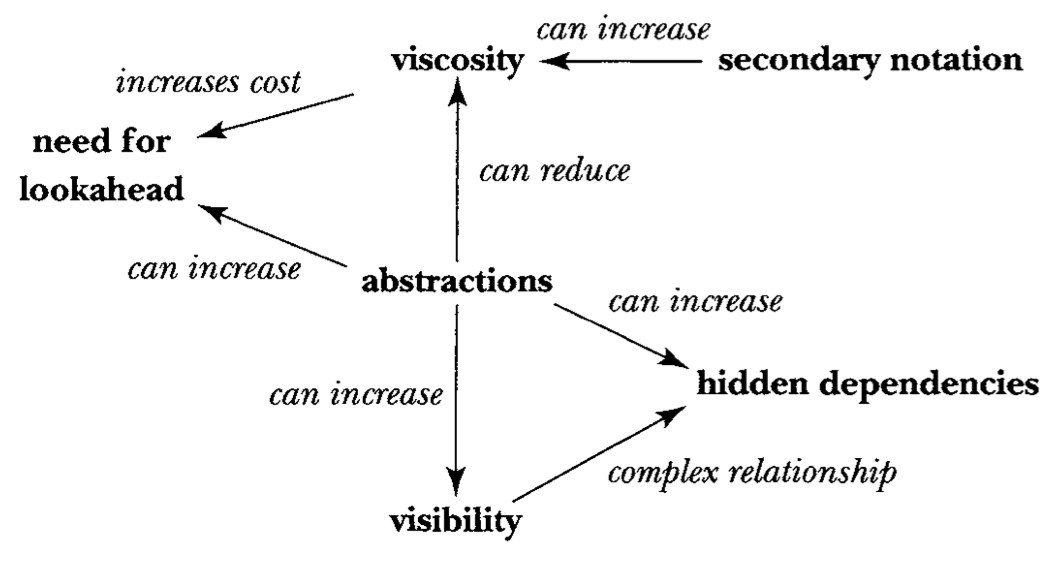
\includegraphics[width=0.7\textwidth]{Figures/CD-TradeOffs.png}
  \caption{Typische Abhängigkeiten zwischen kognitiven Dimensionen.\\\citep{carroll2003hci}}
  \label{fig:CDTradeOffs}
\end{figure}




\section{API-Usability-Evaluation}
\label{sec:api-usability-evaluation}

Dieser Abschnitt befasst sich mit Usability-Evaluationsmethoden der besonderen Art. Nun besteht die Schnittstelle nicht mehr zwingend aus einer grafischen Benutzeroberfläche, sondern aus einer \acrshort{api}{API}.

Aus diesem Grund spielen die im \sref{sec:definitions} eingeführten Begriffe \textit{API-Entwickler}, \textit{API-Anwender} und \textit{API-Endanwender} im Folgenden eine wichtige Rolle.

\subsection{End-User Programming \& End-User Software Engineering\\(Ko u.a. 2011)}
\label{sec:euse}

\begin{important}
\textit{Diese Arbeit ist relevant für ein korrektes Verständnis der SeqAn-Anwenderschaft, zu denen neben API-Anwendern auch API-Endanwender gehören.}

\cite{Ko:2011el} haben in ihrer lesenswerten Literaturstudie ``The State of the Art in End-User Software Engineering'' einen umfassenden Überblick über den Bereich der \textit{Endanwender-Softwaretechnik} (EUSE) gegeben. Häufiger ist in der Literatur jedoch von \textit{Endanwender-Programmierung} (engl. \textit{end-user programming}) die Rede. Betrieben wird sie von \textit{Endanwender-Programmierern} (engl. \textit{end-user programmers}), zu denen Künstler, Architekten, Wissenschaftler, aber auch System-Administratoren gehören können.

Definiert werden Endanwender-Programmierer als Personen, deren Ziel nicht das Programmieren ist, sondern das Programmieren ein ``notwendiges Übel'' zur Erreichung eines Ziels in ihrer Expertendomäne ist. Die Einordnung von Wissenschaftlern der Bio- oder Wirtschaftsinformatik macht diese lose Definition nicht unbedingt leicht. Daher schlagen \cite{Ko:2011el} vor, das Unterscheidungskriterium der \textit{Zielgruppe} zu verwenden. Das bedeutet, je mehr eine Person für sich, und damit nicht für andere programmiert, desto eher handelt es sich um einen Endanwender-Programmierer (siehe \fref{fig:euse}).

Hat sich die Endanwender-Programmierungsforschung zunächst auf Tabellenkalkulationen und imperative ereignisbasierte Sprachen konzentriert, traten später immer mehr Plattformen, Paradigmen und Softwaretechnikpraktiken in den Fokus der Forschung. Es hat sich gezeigt, dass Endanwender-Programmierer mit allen Bereichen der Softwaretechnik, ob bewusst oder unbewusst, konfrontiert sind. Aus diesem Grund setzt sich immer häufiger der Begriff der Endanwender-Softwaretechnik (EUSE) durch. Die Vorstellung, Endanwender-Programmierer beschränken sich auf die Verwendung von Tabellenkalkulationen, ist überholt. Auch anspruchsvollere Programmiersprachen wie C{}\verb!++! können zum Gebrauch kommen. 

Eine besonders extreme, in \tref{tab:diff-euse-activities} dargestellte Beobachtung in Bezug auf Endanwender-Programmierer ist, dass sie sich durch ein opportunistisches (vgl. \sref{sec:personas}) und mit einem übersteigerten Selbstbewusstsein geprägtes Verhalten auszeichnet. So werden teils offensichtlich falsche, aber durch ein selbstgeschriebenes Programm berechnete, als korrekte und nicht zu überprüfende Ergebnisse angesehen.

Ein zweite, besonders erwähnenswerte Beobachtung ist, dass für den eigenen Bedarf entwickelte Anwendungen unerwartet oft von Kollegen verwendet und weiterentwickelt werden. Die Anwendung entwickelt sich damit in Richtung Standardsoftware, was durch die unzureichende Beachtung von softwaretechnischen Erkenntnissen und Praktiken wiederum zu Problemen führt \citep{Letondal:2006dy,Ko:2011el}. Im Grunde unterscheidet sich die Endanwender-Softwaretechnik von der Softwaretechnik darin, dass die eingesetzten, den Qualitätsaspekten betreffenden Aktivitäten nicht oder nur sekundär verfolgt werden \citep{,Ko:2011el}.

\begin{center}
  \begin{tabularx}{\linewidth}{X X X}
  \textbf{Softwaretechnik-Aktivität} & \textbf{Professionelle Softwaretechnik} & \textbf{Endanwender-Softwaretechnik} \\
  \midrule
  Anforderung & explizit & implizit \\
  Spezifikation & explizit & implizit \\
  Wiederverwendung & geplant & ungeplant \\
  Test / Verifikation & vorsichtig & übersteigertes Selbstbewusstsein \\
  Debugging & systematisch & opportunistisch \\
  \end{tabularx}
  \captionof{table}[Qualitative Unterschiede zwischen professioneller und Endanwender-Softwaretechnik]{Qualitative Unterschiede zwischen professioneller und Endanwender-Softwaretechnik \citep{Ko:2011el}}
  \label{tab:diff-euse-activities}
\end{center}

%Abschließend fassen \cite{Ko:2011el} zusammen, dass sich die EUSE-Forschung zuletzt auf die Bereiche Web und Anwendungsdomäne konzentrierte.
\end{important}

\begin{figure}
  \centering
    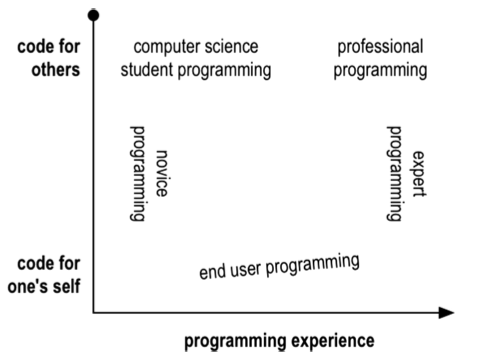
\includegraphics[width=0.5\linewidth]{Figures/end-user-programming.png}
    \caption{Einordnung von Endanwender-Programmierern entlang der Dimensionen \textit{Programmiererfahrung} und \textit{Zielgruppe}}
    \label{fig:euse}
\end{figure}



\subsection{Klassische Usability-Evaluation}

\cite{Beaton:2008ix} diskutiert in seiner Arbeit, inwiefern die weiter oben genannten klassischen Usability-Evaluationsmethoden und -techniken zur Evaluation von APIs eingesetzt werden können.

\subsubsection{Think-Aloud-Protokoll}

Diese von \cite{Beaton:2008ix} als ``gold standard'' bezeichnete HCI-Technik findet häufig Einsatz bei der Evaluation von APIs. Da die Verwender einer API in der Beobachtung beliebige Äußerungen machen können, ist das erfasste Spektrum entsprechend breit und damit die Evaluation schwierig und zeitraubend.

Um dieses Problem zu lösen, schlagen \cite{Stylos:2007jb,Ellis:2007kv} vor, diese Technik nur bei einfachen Aufgaben anzuwenden. Dies ist zugleich auch ein Nachteil, da Probleme, die nur in komplexen Szenarien auftreten, unentdeckt bleiben. Ein cleveres Verfahren in einer der Arbeiten \citep{Ellis:2007kv} möchte ich hier unerwähnt lassen: Anstatt Entwickler direkt ein Problem in echten Quellcode lösen zu lassen, sollten sie das Problem zunächst mit Pseudocode lösen. Damit fiel es ihnen viel leichter, auf das mentale Modell der Entwickler zu schließen.

Für quantitative Betrachtungen schlagen \cite{Ellis:2007kv,Beaton:2008ix} vor, die Zeit bis Erfüllung der Aufgabe als Maß für die API-Usability zu nehmen.


\subsubsection{Heuristische Evaluation}
\begin{important}
\textit{Die Heuristische Evaluation wird im \sref{sec:phase1} für eine erste Analyse der SeqAn-API verwendet.}

\cite{Nielsen:1990bw} formuliert zehn Heuristiken, die sich dazu eignen, Usability-Probleme durch Experten zu finden. Dieser Ansatz erkennt zwar nicht alle Usability-Probleme, zeichnet sich aber durch seine einfach Handhabung und Kosteneffizienz aus.

\cite{Beaton:2008ix} schlagen vor, diese Heuristiken auch zur Evaluation der API-Usability zu verwenden. Dabei sollen die Heuristiken \textit{consistency and standards}, \textit{error prevention} und \textit{help and documentation} besonders relevant sein --- eine Einschätzung, die ich ebenfalls teile.

Speziell zur Evaluation von API-Usability gibt es nur eine Heuristikauflistung \citep{Grill:2012jm}, die allerdings konstruktive Mängel aufweist und auf die ich im Ausblick eingehe.

Ein zweiter Vorstoß kommt von \cite{Watson:2012es}, der systematisch drei Heuristiken zur Bewertung von API-Dokumentation entwickelt und validiert hat. Diese lauten Ersteindruck (engl. \textit{initial impression}), Erlebnis (engl. \textit{experience}) und zusätzliche Daten (engl. \textit{additional data}). Auf diese Heuristiken gehe ich im \sref{sec:improve-dox} genauer ein.

Etwas weniger praktisch anwendbar sind die von \cite{Correia:2010bx} vorgestellten Muster für eine konsistente API-Dokumentation, die in der Forschung leider wenig Beachtung fanden. In den Arbeitsergebnissen sehe ich das Potential, dass sie als Grundlage für Heuristiken für die Evaluation von API-Dokumentationen dienen können.

Abgesehen von den eben genannten Arbeiten konnte ich in der Literatur keine weiteren Forschungsergebnisse zu API-Heuristiken finden.
\end{important}


\subsubsection{Cognitive Walkthrough}

Bei der Anwendung des Cognitive-Walkthrough-Verfahrens \citep{Wharton:1994to} werden Annahmen über die idealtypischen Benutzer gemacht, deren Beschreibung sich in Form von Personas (vgl. \sref{sec:personas}) anbietet. Dies ist eine Stärke in Bezug auf APIs, wenn die Nutzerschaft unbekannt oder wegen des frühen API-Entwicklungsstandes noch nicht bekannt ist.

Das Cognitive-Walkthrough-Verfahren sieht vor, dass das Evaluatorenteam Anwendungsszenarien beschreibt, deren Erfüllungsgrad durch die Anwendung an Hand von vier Fragen überprüft wird. Diese Fragen werden in ihrer Form von \cite{Beaton:2008ix} als nicht verwendbar beschrieben, da die Entwicklung mit einer API viel mehr Freiheitsgrade zulässt als bei der Verwendung eines Endanwender-Programms. Daher reformulierten \cite{Beaton:2008ix} die Fragen wie folgt:

\begin{itemize}
  \item Welches Ziel hat der Benutzer, wenn ihm dieses Szenario präsentiert wird?
  \item Welche Optionen werden von dem Benutzer wahrgenommen?
  \item Welche wahrgenommenen Optionen scheinen am meisten umsetzbar?
  \item Welches Ergebnis wird der Benutzer erreichen?
\end{itemize}



\subsubsection{Cognitive Dimensions Framework}
\label{sec:api-cds}

\begin{important}
\textit{Dieser Abschnitt ist relevant für den im \sref{sec:phase2} vorgestellten Cognitive-Dimensions-Fragebogen und für den in \href{sec:Ergebnisse}{Kapitel 4} unternommenen Versuch der Validierung meiner Ergebnisse.}

Trotz des engagierten und nicht ganz unerfolgreichen Versuchs von \cite{161956}, einen generischen CD-Fragebogen zu erarbeiten, konzentrierten sich andere Arbeiten auf eine Spezialisierung der CDs. Zu den relevantesten Arbeiten gehört ``Using the Cognitive Dimensions Framework to evaluate the usability of a class library'' von \cite{Anonymous:9HSMlhmF}. Wie der Name schon sagt, haben die Autoren in ihrer Arbeit Greens CDs so angepasst, dass sie sich in besonderer Weise zur Evaluation von APIs eignen. Dies schließt auch etwaige Dinge wie Programmiersprache, Entwicklungsumgebung, Debugging-Werkzeuge und Dokumentation ein.

Die Anpassung der CDs geschah auf zweierlei Weise:
\begin{description}
\item[Terminologie] Clarke und Becker haben die generische Terminologie so deduziert, dass sie von API-Entwicklern verstanden wird. Dabei entfiel insbesondere der Term \emph{Notation}, welcher durch \emph{\acrshort{api}} ersetzt wurde.
\item[Dimensionen] Abgesehen von der Benennung waren manche Dimensionen auch inhaltlich nicht angemessen für die Evaluation von API. Darüber hinaus liegt es auf der Hand, dass es auch CDs geben kann, die nicht Teil der von Green vorgeschlagenen CDs sind. Letzteres Problem haben die Autoren auf interessante Weise gelöst: Sie haben bereits API-Usability-Tests mittels Videoaufzeichnung und anschließender Auswertung durchgeführt und ``signifikante Verbesserungen'' erreicht. Teile der Ergebnisse waren allerdings nicht durch die CDs von Green herzuleiten und wurden daher als Grundlage zur Formulierung weiterer CDs verwendet.
\\\\
Eine prominente neue Dimension heißt \emph{Work-Step Unit}. Sie beschreibt, wie viel Arbeit durch eine typische Codezeile gelöst wird.
\end{description}

Die von Clarke entwickelten 12 CDs lauten wie folgt:
\begin{description}
\item[Abstraktionsebenen (\textit{Abstraction Level})] Wie lauten die von der API angebotenen minimalen und maximalen Abstraktionsebenen? Sind sie für die Zielgruppe nutzbar?
\item[Lernanforderungen (\textit{Learning Style})] Welche Lernanforderungen werden durch die API an den API-Anwender gestellt? Welche Lerntypen werden unterstützt?
\item[Arbeitsgedächtnisanforderungen (\textit{Working Framework})] Wie viele konzeptuelle Informationen / Chunks muss der API-Anwender im Kopf behalten, um mit der API effektiv arbeiten zu können?
\item[Arbeitsschrittgröße / Codedichte (\textit{Work-Step Unit})] Welcher Umfang einer Programmieraufgabe wird durch einen einzelnen Schritt (i.d.R. ein Statement) erledigt?
\item[Fortschreitende Evaluation (\textit{Progressive Evaluation})] In welchem Umfang kann teilweise vollständiger Code ausgeführt werden, um Feedback zum Programmverhalten zu erlangen?
\item[Verfrühter Entscheidungszwang (\textit{Premature Commitment})] In welchem Umfang muss der API-Anwender Entscheidungen treffen, bevor ihm alle dafür notwendigen Informationen vorliegen.
\item[Durchdringbarkeit (\textit{Penetrability})] In welchem Umfang wird der API-Anwender unterstützt, die Komponenten der API zu explorieren, zu analysieren und zu verstehen? Wie gelangt der API-Anwender an diese Informationen?
\item[API-Anpassungnotwendigkeit (\textit{API Elaboration})] In welchem Umfang muss die API angepasst werden, um die Bedürfnissen eines API-Anwenders zu erfüllen?
\item[Anpassungsfreundlichkeit (\textit{API Viscosity})] Wie schwierig und aufwändig sind inhärente Änderungen am auf der API basierenden Code?
\item[Konsistenz (\textit{Consistency})] Inwiefern kann über die API erlerntes Wissen auf den Rest der API übertragen werden?
\item[Rollenerkennbarkeit (\textit{Role Expressiveness})] Wie einfach ist die Rolle einer Komponente innerhalb der API als Ganzes zu erkennen?
\item[Problementsprechung (\textit{Domain Correspondence})] Wie deutlich hat eine API-Komponente eine Entsprechung in der Problemdomäne.
\end{description}

Die Autoren betonen, dass diese Aufzählung nicht vollständig ist, da sie aus lediglich einer API-Usability-Studie extrahiert und an Hand von drei Studien validiert wurde. Dennoch finden diese API-CDs bereits regen Gebrauch beim Arbeitgeber der Autoren (Microsoft) und konnten bereits nachweislich API-Verbesserungen verbuchen.

Allerdings sind Clarkes API-CDs nicht vollständig nachvollziehbar. Clarke entfernte beispielsweise die \acrshort{cd} \textit{error-proneness}, obwohl diese für die Diskussion von Notationen im Softwarebereich von \cite{Blackwell:1999vi} als eindeutig hilfreich eingestuft wird. Gleiches gilt für die \acrshort{cd} \textit{juxtaposability}. Diese \acrshort{cd} kann am besten mit Gegenüberstellbarkeit übersetzt werden. In dem Artikel von \cite{Blackwell:1999vi} wird ein Beispiel genannt, in dem ein Diagramm in Code übersetzt wird (Aktivität: Transkription) und die Anwenderin Diagramm und Code gleichzeitig sehen wollte. An dieser Stelle könnte man das Argument ins Feld führen, dass \cite{Blackwell:1999vi} von Programmiertätigkeiten im Allgemeinen und \cite{Anonymous:9HSMlhmF} konkret von der Arbeit mit \acrshort{api}s sprechen. Ich halte die Kürzung aber für einen Fehler, da man sich für beide \acrshort{cd}s problemlos Beispiele vorstellen kann, die im Kontext von \acrshort{api}s relevant sind.

Ich konnte exakt zwei Anwendungen von Clarkes API-CDs in der Literatur finden:

Die erste Anwendung findet bei \textit{Microsoft} in Form einer API-Usability-Evaluationsmethode statt. In zwei Nachträgen \citep{Clarke:2003wk,clarke:2006} erklärt Clarke, wie dabei verfahren wird:
\begin{itemize}
\item Für die Erhebung der CDs einer API werden fünf API-User eingeladen, um API-relevante Aufgaben zu lösen.
\item Dabei werden die Teilnehmer verschiedenartig beobachtet. Zu den typischen Beobachtungsverfahren gehören Think-Aloud, Beobachtung durch einen semi-transparenten Spiegel und Videoaufzeichnungen.
\item Für die Erledigung der Aufgaben hat jeder Entwickler 2h Zeit.
\item Die Beobachtungen werden von Spezialisten ausgewertet und ein CD-Profil wird erstellt.
\item \cite{Stylos:2007jb} haben drei Personas entwickelt (\textit{Opportunisten}, \textit{Pragmatiker} und \textit{Systematiker}), auf die ich näher im \sref{sec:personas} eingehe. Für jede Persona existiert ein vorab erstelltes CD-Idealprofil.
\item Das erstellte CD-Profil wird mit den Idealprofilen der Personas verglichen, die am ehesten der Zielgruppe entsprechen.
\item Je mehr sich die CD-Profile gleichen, desto höher ist die Usability.
\item Die CDs selbst werden dann als Diskussionsgrundlage verwendet, um eine zielgerichtete Anpassung des CD-Profils zu erreichen.
\end{itemize}

Leider halten sich die beiden Arbeiten in den Details auffällig zurück. Es wird weder darauf eingegangen, wie die drei Idealprofile nun konkret aussehen, noch, mit welchem Erfolg die CDs eingesetzt wurden.

Die zweite Anwendung findet sich in der empirischen Arbeit von \cite{Piccioni:2013uq}. Unter anderem wurden die Probanden dieser Studie mit einem Fragebogen konfrontiert. Laut der Autoren basiert dieser auf Clarkes API-CDs. Kritisch sehe ich an deren Vorgehen folgende Punkte:
\begin{enumerate}
  \item Die Autoren zeigen nicht, welche der gestellten Fragen sich auf welche kognitive Dimension stützt. Obwohl ich mich intensiv mit dem \gls{cdf} auseinandergesetzt habe, gelang es mir nicht, eindeutig diese Bezüge herzustellen.
  \item Offensichtlich werden nicht alle CDs durch die Fragen abgedeckt. Unter den Fragen, die ich eindeutig auf die jeweilige CD beziehen konnte, gab es zwei, die auf dieselbe CD abzielten. Da es 12 API-CDs und 12 Fragen gab, muss gemäß dem Taubenschlagprinzip mindestens auf eine CD verzichtet worden sein. Da die Autoren den Anspruch formulierten, neue problematische API-Usability-Aspekte zu ermitteln, sehe ich es kritisch, die erfragten CDs zu kürzen. 
\end{enumerate}

Zusammenfassend stelle ich fest, dass \cite{Piccioni:2013uq} das \gls{cdf} in seinem ursprünglichen Sinne, nämlich als Diskussionswerkzeug, verwenden. Die Verwendung als API-Usability-Evaluationsmethode wird lediglich in \cite{Clarke:2003wk,clarke:2006} beschrieben --- das allerdings unzureichend.

Im \sref{app:cdf} gebe ich einen Ausblick auf Weiterentwicklungsmöglichkeiten des \gls{cdf} im Allgemeinen und seiner Anwendung als Evaluationsmethode für APIs im Speziellen.
\end{important}



\subsection{Personas (Clarke 2007)}
\label{sec:personas}

\begin{important}
\textit{Die von Clarke entwickelten Personas sind relevant für die in \href{sec:Ergebnisse}{Kapitel 4} vorgestellten \code{apiua://code/-9223372036854775414}, die ich bei den SeqAn-Anwendern beobachten konnte.}

Für die Evaluation von Usability und damit auch von API-Usability ist ein Verständnis des Benutzers selbst notwendig \citep{Sarodnick:2006vc}. Die Anforderung ist leicht zu erfüllen, wenn es sich um Individualsoftware bzw. eine individuelle API handelt. Sprechen wir aber von Standardsoftware, sind Nutzergruppen mannigfaltig und schwer zu erfassen.

Personas sind Personenbeschreibungen von Repräsentanten verschiedener Nutzergruppen und eignen sich als Alternative zum szenariobasierten Interaktionsdesign. Eine Persona ist facettenreich und ihre Beschreibung umfasst mehr als die Aufzählung ihrer demographischen Werte \citep{Pruitt:2003ki}. Dabei hat die Glaubwürdigkeit einer solchen Beschreibung Vorrang vor Diversität und politischer Korrektheit\footnote{\cite{Cooper:1999vg} nennt ein amüsantes Beispiel, dass ich Ihnen nicht vorenthalten möchte: Zur Beschreibung eines Computertechnikers zieht er die Persona Nick --- ein pickeliges 23jähriges Ex-Mitglied der Technik-AG seines damaligen Gymnasiums --- der Persona Hellene --- einer klassischen 1,80m großen Schönheit der Beverly Hills High --- vor.} \citep{Cooper:1999vg}.

\cite{Stylos:2007jb,clarke:DSP:2007:1080} haben die folgenden drei --- nicht ganz stereotypfreien --- Personas entwickelt, die sich zur Evaluation von Standard-APIs eignen:
\begin{description}
\item[Opportunistische Entwickler] arbeiten \textit{bottom-up} und möchten sich nicht mit Low-Level-Problemen auseinandersetzen. Sie möchten ihren Code schnell zum laufen bringen, ohne ein tieferes Verständnis von der zugrunde liegenden API zu erlangen.
\item[Pragmatische Entwickler] sind defensiver und lernen ``unterwegs''. Sie arbeiten wie opportunistische Entwickler \textit{bottom-up}. Sollte diese Strategie scheitern, wechseln sie zu \textit{top-down}, um ein besseres Verständnis zu erhalten. Sie wägen gerne Einfachheit und Kontrolle ab. Beispielsweise verwenden pragmatische Entwickler häufig gern grafische Code-Editoren. Dennoch möchten sie über die Option verfügen, den automatisch erstellten Code nachbearbeiten zu können. Typischerweise präferierte Sprachen sind Java und C\#, die ein ausgewogenes Verhältnis zwischen Einfachheit und Kontrolle bieten.
\item[Systematische Entwickler] arbeiten \textit{top-down} und versuchen, ein Gesamtverständnis vom System zu erhalten, bevor sie sich auf eine Komponente konzentrieren. Sie programmieren defensiv und machen wenig Annahmen über den Code / der API. Sie misstrauen den Garantien, die eine \acrshort{api} macht und testen lieber die Funktionstüchtigkeit in der eigenen Umgebung. Sie möchten nicht nur verstehen, ob, sondern auch warum der Code läuft, welche Annahmen er macht und wann er versagen könnte. Sie ziehen Sprachen wie C++, C oder Assembler vor, die ihnen eine hohe Kontrolle erlauben.
\end{description}

Die Beschreibungen lassen sich mit den Erkenntnissen von \cite{Shaft:1998tc} in Einklang bringen. Zur Erinnerung: Die Arbeit integrierte die Ergebnisse von \cite{Brooks:1983fj} und \cite{Pennington:1987dc}, indem sie die Domänenkenntnisse der Entwickler mit in Betracht zog. Demnach beobachtet man bei Entwicklern mit wenig Domänenkenntnissen, dass diese häufig ein Bottom-Up-Vorgehen anwenden. Entwickler, die über viele Domänenkenntnisse verfügen, benutzen häufiger ein Top-Down-Vorgehen. Diese Herangehensweise wird als \textit{flexibel} bezeichnet und entspricht damit der Pragmatischer-Entwickler-Persona.
\\ Entwickler mit einer unflexiblen Herangehensweise hingegen wenden immer das Top-Down- bzw. das Bottom-Up-Vorgehen an, entsprechen also der Systematischer-Entwickler- bzw. Opportunistischer-Entwickler-Persona.
\\ Umgekehrt ausgedrückt hieße das: Bei opportunistischen und systematischen Entwicklern spielen die Domänenkenntnisse keine Rolle bei der Wahl der Herangehensweise --- aber für den Erfolg. Pragmatische Entwickler präferieren das Bottom-Up-Verfahren und wechseln --- abhängig von auftretenden Problemen und ihren Kenntnissen der Domäne --- zum Top-Down-Verfahren.   

Schreibt man einer realen Person eine anders definierte Persona zu, muss man damit rechnen, dass diese Zuschreibung nicht immer gilt bzw. sich über die Zeit verändert. Dies ist der Fall, wenn Personas über das Alter, die Erfahrung oder den Beruf definiert sind, was bei Langzeitbeobachtungen problematisch sein kann.

Die drei von \cite{Stylos:2007jb} beschriebenen Personas leiden weniger unter dieser Gefahr, da sie unabhängig von Beruf, Expertise, Ausbildung und Erfahrung gelten \citep{clarke:DSP:2007:1080,Stylos:2006td}.
Für die Sinnhaftigkeit und Anwendbarkeit dieser Personas spricht, dass sie die Beobachtungen von \cite{Shaft:1998tc} ergänzen und in verschiedenen API-Usability-Arbeiten erfolgreich angewandt wurden \citep{Stylos:2007jb,Stylos:2008cu,Stylos:2008jt}. \cite{clarke:DSP:2007:1080} nutzte diese Personas bereits vier bis fünf Jahre vor ihrer Veröffentlichung für seine Forschung.
\end{important}


\subsection{Metriken (Stylos u. Myers 2007)}

\begin{important}
\textit{Diese Arbeit ist relevant für die in \href{sec:Ergebnisse}{Kapitel 4} vorgenommene Unterteilung von \code[apiua://code/-9223372036854775281]{Entwurfsentscheidungen}.}

\cite{Stylos:2007ip} haben sich im Rahmen ihrer Arbeit Expertenmeinungen, komparative Laborstudien, informelle Onlinediskussionen und Forschung zum Thema objektorientierte Programmierung angesehen und die vielen ungeordneten, sich teils überlappenden oder gar synonymen Qualitätsfaktoren/-merkmale/-eigenschaften verglichen. Die gefundenen Qualitätsfaktoren wurden zu den folgenden drei Kategorien (vgl. \fref{fig:APIQualityHierarchy}) zusammengefasst. Metriken, mit denen sich die Qualitätsfaktoren messen lassen, erläutert die Arbeit nicht.
\begin{description}
  \item[Stakeholders] \hfill \\
  Bestehen aus den Entwicklern und Anwendern der API sowie aus den Verbrauchern der durch die API-Anwender entwickelten Programme.
  \item[Usability] \hfill \\
  Diese Qualitätsfaktoren beeinflussen das Erzeugen und Debuggen des von API-Anwendern entwickelten Codes.
  \item[Mächtigkeit] \hfill \\
  Diese Qualitätsfaktoren betreffen Beschränkungen des von API-Anwendern entwickelten Codes.
\end{description}

Für meine Arbeit ist ein anderer Beitrag der Autoren wichtig. \cite{Stylos:2007ip} schlagen zwei Perspektiven vor, unter denen API-Design-Entscheidungen geordnet werden können (\fref{fig:APIDesignDecisions}). Die erste Perspektive unterscheidet zwischen Design-Entscheidungen auf Architektur- bzw. Sprachebene. Die zweite Perspektive unterscheidet zwischen strukturellen Design-Entscheidungen und solchen auf Klassenebene. 

\cite{Stylos:2006td,Stylos:2007ip} kritisieren, dass viele in der Literatur gefundenen Entwurfsempfehlungen (z.B. ``Returning null versus returning an empty object
(i.e., an empty string).'') nie von den jeweiligen Autoren überprüft wurden und teilweise widersprüchlich sind.

Verschiedene Design-Entscheidungen haben unterschiedliche Prioritäten für ihre Behebung --- abhängig von ihrem Einfluss auf die Eigenschaften der API. \cite{Stylos:2006td} nennen drei Dimensionen, über die sich die Priorität herleiten lässt:
\begin{itemize}
\item Die \emph{betroffene Partei} - also sind API-Entwickler oder API-(End-)Anwender von der Designentscheidung betroffen.
\item Die \emph{Frequenz}, mit der man von einer Designentscheidung konfrontiert wird.
\item Die \emph{Schwierigkeit} des Umgangs mit einer Designentscheidung.
\end{itemize}

Aus dem besser erforschten Gebiet der klassischen (Nicht-API-)Usability kommt noch eine weitere Dimension dazu, die von \cite{Nielsen:1994tx} als \emph{Persistenz} bezeichnet wird. Persistenz beschreibt, ob ein Usability-Problem bei erneutem Auftreten auch immer wieder aufs Neue als störend empfunden wird. Darüber hinaus schlagen \cite{Sarodnick:2006vc} \emph{Markteinfluss} als boolesche Eigenschaft vor. Diese Eigenschaft ist lediglich relevant, wenn die Nicht-Behebung eines Problems kommerzielle Folgen, z.B. durch Nicht-Verkauf des Produkts, wahrscheinlich macht.
\end{important}

\begin{figure}
  \centering
    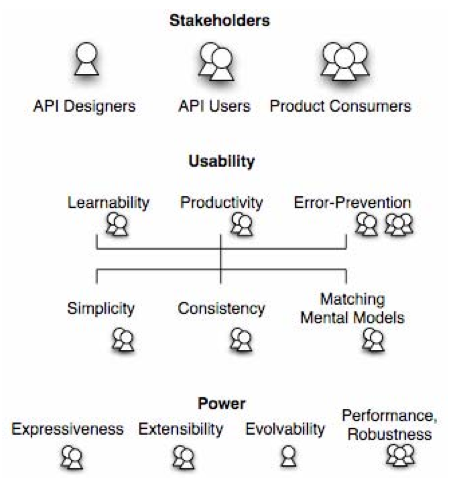
\includegraphics[width=0.5\textwidth]{Figures/APIQualityHierarchy.png}
  \caption{Qualitätseigenschaften von APIs \citep{Stylos:2007ip}}
  \label{fig:APIQualityHierarchy}
\end{figure}

\begin{figure}
  \centering
    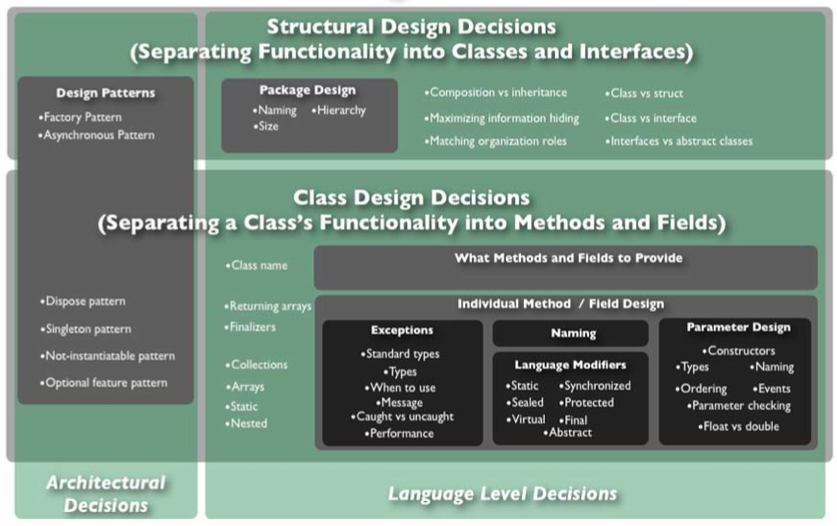
\includegraphics[width=1.0\textwidth]{Figures/APIDesignDecisions.png}
  \caption{Kategorisierung von API-Designentscheidungen \citep{Stylos:2007ip}}
  \label{fig:APIDesignDecisions}
\end{figure}






\subsection{Lernbarrieren (Ko u.a. 2004)}

\cite{AndrewJKo:2004df} haben 40 Endanwender-Programmier (im Sinne von \acrshort{euse}) beobachtet, die im Begriff waren, die Sprache \textit{Visual Basic.NET} über einen Zeitraum von fünf Wochen zu erlernen. Die Probanden konnten dabei stets auf ein Orakel (einer der Experimentatoren) zurückgreifen, das alle aufgekommenen Fragen beantwortete. Ebenso gaben die Probanden auf Fragen des Experimentators (``Wo hängst du?'', etc.) Antwort.

Ziel war es herauszufinden, durch welche Arten von Problemen das Erlernen erschwert wird (vgl. \fref{fig:learningbarriers1}).

Die Autoren konnten 130 Lernbarrieren ermitteln, die sie zu den folgenden sechs Kategorien zusammenfassen:

\begin{description}
\item[Design Barriers] \textit{``I don’t know what I want the computer to do...''} \hfill \\
  Designbarrieren sind inherent schwierig. Sie zu überwinden, fordert Kreativität. Entwickler des Systems werden von den Autoren aufgefordert, die Kreativität der Endanwender-Programmierer mit Hilfe von Beispielen und anderen Formen zu inspirieren.
\item[Selection Barriers] \textit{``I think I know what I want the computer to do, but I don’t know what to use...''} \hfill \\
  Selektionsbarrieren sind schwierig zu überwinden. Bei diesem Problem kann eine Suchfunktionen helfen, die es erlaubt, nach dem Verhalten von Komponenten zu suchen.
\item[Coordination Barriers] \textit{``I think I know what things to use, but I don't know how to make them work together...''} \hfill \\
  Eine wichtige Größe bei diesem Problemen sind unsichtbare Regeln, deren Existenz und Nichteinhaltung häufig nur durch Fehlerausgaben sichtbar gemacht wird. \cite{dekel2011increasing} hat eine Möglichkeit vorgestellt, wie dieses Problem weitgehend gelöst werden kann (siehe \sref{sec:api-directives}).
\item[Use Barriers] \textit{``I think I know what to use, but I don't know how to use it...''} \hfill \\
  Gebrauchsbarrieren treten sehr schnell auf. Ursachen sind die mangelhafte Dokumentation des Interfaces. Besonders wichtig zu dokumentieren sind Feedback und Beschränkungen von Funktionen. Die textuelle Repräsentation von Systemen erschwert Endanwender-Programmierern deren Erlernen.
\item[Understanding Barriers] \textit{``I thought I knew how to use this, but it didn’t do what I expected...''} \hfill \\
  Verständnisbarrieren gehen auf fehlende Erklärungen zurück, die Auskunft geben, was das Programm getan bzw. nicht getan an. Nachvollziehbarkeit wird als Hauptursache genannt.
\item[Information Barriers] \textit{``I think I know why it didn’t do what I expected, but I don’t know how to check...''} \hfill \\
  Nachvollziehbarkeit wird auch für Informationsbarrieren als Hauptursache genannt.
\end{description}

Problematisch werden Lernbarrieren, wenn eine Person falsche Annahmen zur Überwindung der Barriere trifft. Dies kann dazu führen, dass der Anwender ein falsches Verständnis von der zu erlernenden Sprache erwirbt, die ihn ultimativ darin hindert, weitere Barrieren zu überwinden. Diese werden von den Autoren als \textit{unüberwindbar} bezeichnet (siehe \fref{fig:learningbarriers2}).

\cite{AndrewJKo:2004df} argumentieren, dass die ermittelten Lernbarrieren auch auf professionelle Entwickler anwendbar sind. Ich schlussfolgere aus der Top-Down-Theorie von \cite{Brooks:1983fj}, dass professionelle Entwickler mit Hilfe der Hypothesenbildungsstrategie und ihrem reicheren Erfahrungsschatz potentiell weniger Probleme bei der Überwindung von Lernbarrieren haben als Endanwender-Programmierer.

Die Anwendbarkeit der Lernbarrieren auf \glslink{api}{APIs} argumentiere ich mit der Vermutung, dass Endanwender-Entwickler nicht hinreichend zwischen Programmiersprache und API unterscheiden. Auch könnte man sagen, dass eine Programmiersprache im Kern eine mögliche Schnittstelle zur Interaktion mit einem Computer darstellt, so wie eine API eine Schnittstelle zur Interaktion mit einer Softwarebibliothek ist. \cite{Green:1989wb} (vgl. \sref{sec:cdf}) würde in beiden Fällen von einer Notation sprechen, die es zu erlernen gilt.

Für die Anwendbarkeit jedoch spricht am meisten, dass ich noch vor der Lektüre dieser Arbeit alle Informationsbarrieren außer der Koordinationsbarriere in meinen Daten finden konnte\citepurl{apiua://code/-9223372036854774911}.

\begin{figure}
  \centering
    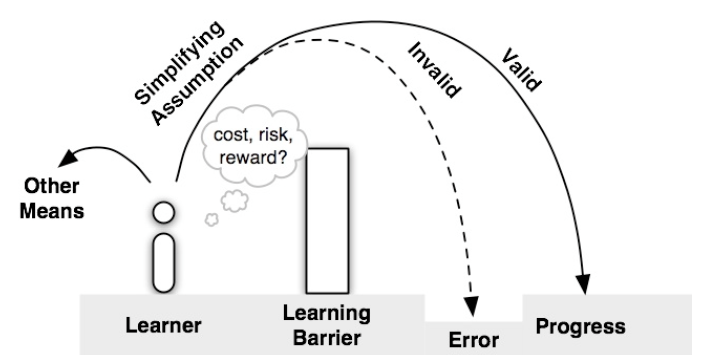
\includegraphics[width=0.55\linewidth]{Figures/learningbarriers1.png}
  \caption[Lernbarriere --- Treffen einer Annahme]{Beim Überwinden einer Lernbarriere riskieren Erlerner, eine falsche Annahme zu treffen.}
  \label{fig:learningbarriers1}
\end{figure} 

\begin{figure}
  \centering
    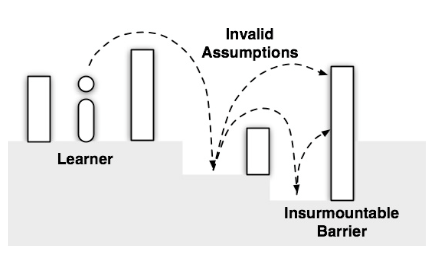
\includegraphics[width=0.45\linewidth]{Figures/learningbarriers2.png}
  \caption[Lernbarriere --- Unüberwindbare Barrieren]{Treffen Erlerner beim Überwinden von Lernbarrieren falsche Annahmen, führt dies häufig zu unüberwindbaren Barrieren.}
  \label{fig:learningbarriers2}
\end{figure} 



\subsection{Abstrakte API-Aktivitäten (Stylos 2009)}

\begin{important}
\textit{Die Dissertation von Stylos ist besonders relevant für die in den Abschnitten \ref{sec:dox} und \ref{sec:improve-dox} vorgestellte Überarbeitung der SeqAn-Dokumentation.}

In seiner Dissertation ``Making apis more usable with improved api designs, documentation and tools'' fasst \cite{Stylos:2009ts} seine jahrelange Forschung zusammen und stellt sein Verständnis vom Erlernen/Gebrauch von Java-basierten APIs vor. Dabei spielen folgende in \fref{fig:high-level-programming-activities} dargestellten Aktivitäten eine Rolle:

\begin{description}
  \item[(A) Initiale Designideen] \hfill \\
  Bei dieser Aktivität entwickelt der API-Anwender ein erstes Verständnis darüber, wie er ein zuvor formuliertes Problem programmatisch lösen kann.

  \item[(B) Abstraktes API-Verständnis] \hfill \\
  In dieser Phase verschafft sich der API-Anwender einen Überblick über existierende und geeignete \glslink{api}{APIs}. Um diese Phase erfolgreich zu absolvieren, muss jede API einen Überblick über sich geben.
  
  Immer häufiger kommen für diese Phase Suchmaschinen wie Google zum Einsatz. Insbesondere für API-Anwender mit wenig Erfahrung stellt dies einen großen Vorteil dar, da sie nicht mit der sonst notwendigen Terminologie vertraut sein müssen. Konkret nennt \cite{Stylos:2009ts} die Suchphrase  ``creating a form in java'' als Beispiel, denn ``form'' ist in der \gls{java}-Entwicklung ein eher unüblicher Begriff und findet in offiziellen Dokumentationen fast keinen Gebrauch.
  
  \item[(C) Architektonisches Design] \hfill \\
  Nachdem Anwender die abstrakten Elemente einer API angefangen haben zu verstehen, entwickelt sich eine Idee, wie eine konkrete API für die eigene Problemlösung genutzt werden kann.
  
  \item[(D) Auffinden von Methoden] \hfill \\
  Diese Phase besteht darin, die Methoden zu finden, die für die Problemlösung gebraucht werden. Erste Hinweise darauf finden Anwender bereits im Zuge von Tutorials oder anderen Artikeln, die auf relevante Methoden/Funktionen verweisen.
  
  Bei Anwendern von Google konnte \cite{Stylos:2009ts} eine höhere Performanz feststellen, denn die Suchergebnisse boten sowohl Code-Beispiele von Dritten als auch Referenzen die offizielle Dokumentation. So bekamen API-Anwender einen schnellen Eindruck über Anwendungsszenarien und konnten dies gleich mit Hilfe der offiziellen Dokumentation verifizieren.
    
  \item[(E) Auffinden von Beispielen] \hfill \\
  Wurden beim Durchlaufen der vorangegangen Phasen noch keine relevanten Code-Beispiele gefunden, wird die Suche in dieser Phase aufgenommen. Dabei kam wiederum Google häufiger zum Einsatz als die offizielle Dokumentation selbst. Angetrieben wurde diese Suche durch Fragen, wie die folgenden:
  \begin{itemize} 
  \item ``Wie instanziiere ich die zu der Methode gehörende Klasse?''
  \item ``Wie bekomme ich Variablen des Typs, die eine Methode als Parameter verlangt?''
  \item ``An welcher Stelle meines Codes muss ich diese Methode aufrufen?''
  \end{itemize}
  
  \item[(F) Integration von Beispielen] \hfill \\
  Gefundene Beispiele reichten von einer Zeile Code bis hin zu vollständigen Programmen, von denen der gesuchte Teil im besten Fall einen Bruchteil ausmachte. Probleme bei der Integration dieser Beispiele ähneln denen von \cite{Fairbanks:2006jw} (siehe oben). Gelingt es dem Anwender nicht, das Beispiel zu integrieren, sucht er nach einem anderen Beispiel für dieselbe Methode (E), einer anderen Methode (D), ändert seinen Entwurf (C) oder sucht nach einer anderen API (B).
\end{description}

Die Beobachtung, dass Google eine wichtige Rolle in den oben zusammenfassten Phasen spielt, veranlasste \cite{Stylos:2006gu}, selbst ein Suchwerkzeug zu entwickeln. Dieses verwendet Google selbst und bietet im Rahmen von APIs eine treffsichere Suche. Das Werkzeug wird etwas genauer im \sref{sec:mica} vorgestellt.
\end{important}

\begin{figure}
  \centering
    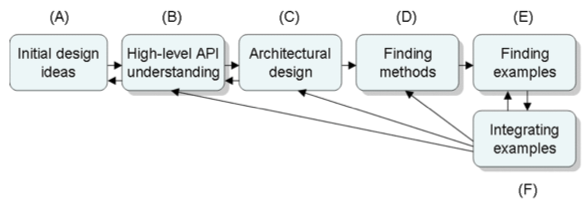
\includegraphics[width=0.9\textwidth]{Figures/high-level-programming-activities.png}
  \caption{Abstrakte Programmiertätigkeiten \citep{Stylos:2009ts}}
  \label{fig:high-level-programming-activities}
\end{figure}



\subsection{API-Direktiven (Dekel 2011)}
\label{sec:api-directives}

\begin{important}
\textit{Diese Arbeit ist relevant für die in den Abschnitten \ref{sec:dox} und \ref{sec:improve-dox} vorgestellte Überarbeitung der SeqAn-Dokumentation.}

\cite{dekel2011increasing} formulierte ``neighbor knowledge awareness''-Probleme als solche, die entstehen, wenn konzeptionell zusammengehörige Entscheidungen und Annahmen über mehrere \emph{Artefakte} (Diagramme, Dokumentation, Quelltext) verteilt sind und später nicht mehr in ihrer Gesamtheit sichtbar gemacht werden.

Beispiel: In einem Objektdiagramm wird die Vererbungshierarchie der \gls{java}-Klassen \texttt{Widget} und \texttt{Button} gezeigt. Dass aber \texttt{super.dispose()} aufgerufen werden muss, wenn die \texttt{dispose}-Methode der \texttt{Button}-Klasse überschrieben wird, findet sich lediglich in der Online-Dokumentation. Wie soll der Entwickler also wissen, ob er über alle relevanten Informationen verfügt? Andererseits würde eine stets vollständige Spezifikation Gefahr laufen, wichtige Details zu verdecken \citep{dekel2011increasing}. 

Natürlichsprachige Aussagen, die solche Entscheidungen, Annahmen, Bedingungen oder Richtlinien einer API betreffen, werden als \emph{API-Direktiven} bezeichnet und haben erst seit kurzem wissenschaftliche Aufmerksamkeit auf sich gezogen \citep{dekel2011increasing,Monperrus:2011bf}. Beispiele für API-Direktiven sind ``must not be null'' und ``not being thread-safe''.

Besonders interessant sind überraschende Klauseln in einer Dokumentation wie die der \gls{java}-Methode \texttt{String.replaceAll(String)}, die den übergebenen String als regulären Ausdruck behandelt, was schnell zu einem unerwarteten Ergebnis führen kann.

\cite{dekel2011increasing} zeigte in seiner Dissertation, dass das Einblenden von API-Direkten an der Stelle, wo das Wissen auch benötigt wird, den Entwicklern ein gezielteres Erforschen tangierender Funktionen ermöglicht. Dieser Ansatz wird von Dekel als \textit{Knowledge Pushing} bezeichnet. Er implementierte dazu ein Eclipse-Plugin namens \textit{eMoose} (\fref{fig:KnowledgePushing}). Das Plugin reichert unter anderem den gelben Eclipse-JavaDoc-Hilfsdialog mit gefundenen API-Direktiven an. Das Plugin wurde lediglich im für die Veröffentlichung notwendigen Umfang implementiert\footnote{In der Arbeit von \cite{dekel2011increasing} musste der Autor die Direktiven manuell erkennen und gruppieren. Außerdem stellte die unzureichende Filterung / Selektion ein Problem dar. Den Anwendern von eMoose wurden stellenweise zu viele Direktiven angezeigt. Neben einfachen Lösungen wie dem Ausblenden einer Direktive, nachdem sie gelesen wurde, macht der Autor auch den Vorschlag, den umgebenden Programmtext mit einzubeziehen.} und seitdem nicht weiterentwickelt\footnote{Stand: 16.03.2015, \url{https://code.google.com/p/emoose-cmu/}}.

\cite{dekel2011increasing} und \cite{Monperrus:2011bf} haben folgende Richtlinien entwickelt, um API-Direktiven von der übrigen Dokumentation zu unterscheiden und exakt zu formulieren:
\begin{itemize}
\item Direktiven müssen ein klar definiertes API-Element identifizieren. So darf beispielsweise eine Klassen-bezogene Direktive nicht von den Methoden dieser Klasse sprechen. \citep{Monperrus:2011bf}
\item Direktiven müssen genau erklären, in welchen Fällen sie relevant sind. \citep{Monperrus:2011bf}
\item Direktiven müssen eine Aktion erfordern oder implizieren. \citep{dekel2011increasing}
\item Direktiven dürfen keine vagen Formulierungen wie ``sollte'' verwenden und stets eine peinlich korrekte Terminologie benutzen. \footnote{Beispiel: Man soll von ``erweitern'' (``extend'') sprechen, wenn \texttt{super.function()} aufgerufen wird bzw. werden muss. Anderenfalls wird ``überschreiben'' (``override'') gesprochen.} \citep{Monperrus:2011bf}
\item Direktiven sollten nicht trivial, erwartet oder üblich sein. \citep{dekel2011increasing}
\item Direktiven sollten relevant für die meisten Aufrufer und Szenarien sein. Anderenfalls würden sie ihre Wirkung verfehlen und erneut vom Wesentlichen ablenken. \citep{dekel2011increasing}
\item Direktiven müssen bei Nicht-Beachtung Konsequenzen haben. Je gravierender die Konsequenzen, desto kleiner darf die Menge von Aufrufern und Szenarien sein. \citep{dekel2011increasing}
\end{itemize}

Basierend auf den Dokumentationen wichtiger \gls{java}-\glslink{api}{APIs} und den Arbeiten von \cite{dekel2011increasing} und \cite{Bruch:il} haben \cite{Monperrus:2011bf} eine Taxonomie von 23 API-Direktiv-Typen entwickelt, die in \fref{fig:APIDirectiveTaxonomy} dargestellt werden.
\end{important}

\begin{figure}[!ht]
  \centering
    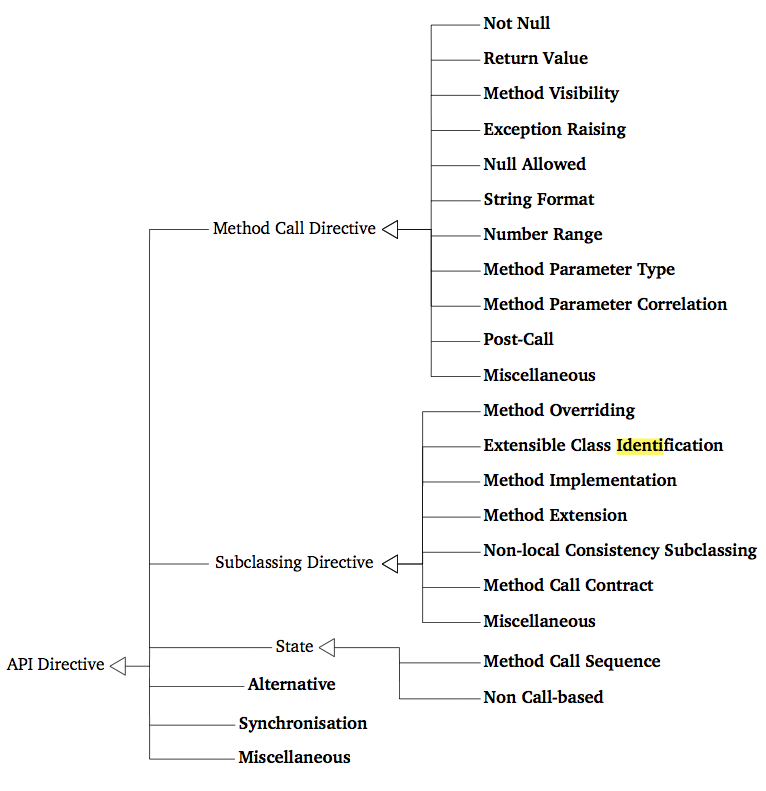
\includegraphics[width=0.75\textwidth]{Figures/APIDirectiveTaxonomy.png}
  \caption{API-Direktiven-Taxononmy \citep{Monperrus:2011bf}}
  \label{fig:APIDirectiveTaxonomy}
\end{figure}





\subsection{Grundlagen / Psychologie / Strategien}

Es fiel mir schwer, für diesen Abschnitt eine gute Überschrift zu finden. Dieser Abschnitt befasst sich mit Beobachtungen, die nicht so recht in die anderen Abschnitte passen wollen, jedoch von durchgängiger Relevanz für meine Arbeit sind.

\subsubsection{Komplizierte Technik (Sarodnick u.a. 2006; Daughtry u.a. 2009a}
\begin{important}
\cite{Daughtry:2009be} haben in ihrer Forschung mehrfach die Beobachtung gemacht bzw. direkt Aussagen dazu gehört, dass Programmieren nun einmal komplizierter ist als der Gebrauch einer grafischen Benutzeroberfläche. Schließlich handele es sich ja um eine Schnittstelle für einen Entwickler und nicht für einen Endanwender.

Ich konnte eine Steigerung dieser Beobachtungen in der Literatur finden \citep{Sarodnick:2006vc}. Dabei geht es darum, dass durch Anwender eines technischen System geäußerte Kritik von den Systementwicklern häufig ``technisch wegargumentiert'' wird. Im Umfeld von API-Usability würde es sich um einen Konflikt zwischen API-Entwicklern und API-(End-)Anwendern handeln, den ich konkret während meiner Forschung beobachten konnte (siehe Abschnitte \ref{sec:gruppendiskussion} und \ref{sec:gt-urursache}).

Das Wissen um dieses Phänomenon ist relevant, wenn der Forscher mit subjektiven Evaluationsmethoden die API-Usability verbessern will.
\end{important}

\subsubsection{Wiederverwendung\\(Lange u. Moher 1989; Rosson u. Carroll 1996; Fairbanks u.a. 2006; Stylos u. Myers 2008)}
\begin{important}
Wiederverwendung ist nicht nur eines der Grundprinzipien von Softwaretechnik, sondern auch eine Strategie, die durch API-(End-)Anwender genutzt wird und sich auch in meinen Forschungsergebnissen zeigt.

Ich konnte in der Literatur zwei Arten der Wiederverwendung in diesem Sinne finden:

\begin{description}
  \item[Implementierungswiederverwendung] \hfill \\
  \cite{Lange:1989jr} haben in ihrer Arbeit einen interessanten Fall beobachtet: Ein erfahrener Entwickler hatte eine existierende Softwarebibliothek, die verschiedene wiederverwendbare Komponenten bereitstellt, um neue Komponenten erweitert. Um dies zu tun, kopierte er häufig eine ähnliche Komponente und passte diese an.
  
  \cite{Rosson:1996da,Stylos:2008jt} machten ähnliche Beobachtungen. Dabei wurden konkret ganze Klassen kopiert und so lange angepasst, bis die angepasste Klasse ihren neuen Zweck erfüllte.
  
  Obwohl diese Form der Wiederverwendung beobachtet wurde, hat keiner der genannten Autoren ihr jemals einen Namen gegeben. Dieser stammt daher von mir.
  
  \item[Anwendungswiederverwendung]\label{sec:reuse-of-uses} \hfill \\
  \cite{Rosson:1996da} beschreiben die Wiederverwendungsform \textit{reuse of uses}, also das Wiederverwenden von Anwendungen. Die Autoren machte die Beobachtung, wie API-(End-)Anwender vor der Frage standen, wie ein bestimmtes API-Konstrukt (Datenstruktur, Funktion, etc.) denn nun genutzt wird. Dazu suchten manche Anwender nach einem ähnlichen Anwendungskontext (z.B. in Form von Code-Beispielen), die dann häufig als verbindliche Vorlage kopiert und angepasst wurden.
  
  Diese Strategie wird von \cite{Fairbanks:2006jw} kritisch gesehen. Sie nennen drei Schwierigkeiten:
  \begin{enumerate}
    \item Das Auffinden solcher konkreten Anwendungsfälle ist schwierig und zeitaufwändig.
    \item Die Bestimmung relevanter Teile ist fehleranfällig.
    \item Die Bewahrung der Intention wird sogar als \textit{unmöglich} (``impossible'') beschrieben.
  \end{enumerate}
  
  \cite{Stylos:2009ts} stellt fest, dass zum Auffinden von Anwendungsfällen immer häufiger die Suchmaschine \textit{Google} zum Einsatz kommt.
\end{description}
\end{important}


\subsubsection{Verständnisvermeidung (Lange u. Moher 1989; Stylos u. Myers 2008)}
\label{sec:Verstandnisvermeidung}

\begin{important}
Dieses Phänomen / diese Strategie ist eines der interessantesten Dinge, die ich überhaupt finden durfte.

\cite{Lange:1989jr,Stylos:2008jt} verstehen darunter die fahrlässige bis aktive Vermeidung, wiederverwendeten Code im Detail zu verstehen. Die Wiederverwendung besteht also im blinden Kopieren und Anpassen vom Code.

Im Sinne von Programmverständnis (vgl. \sref{sec:programmverstandnisforschung}) erklären \cite{Lange:1989jr} damit, dass der Anwender den Code nur \textit{interaktiv}, aber nicht \textit{symbolisch} ausführt.

\cite{Ko:2005cl} beobachten diese Strategie häufig im Kontext von \gls{euse}, was, wegen der potentiell schlechteren Softwaretechnikkenntnisse von API-Endanwendern, leicht nachvollziehbar ist.

\cite{Bruch:2006bv} schildert in seiner Arbeit, dass \glslink{api}{APIs} inherent abstrakter und damit schwerer zu verstehen sind. Schließlich werden \glslink{api}{APIs} mit dem Ziel entworfen, flexibel und für ein breites Spektrum von Anwendungen einsetzbar zu sein. Daher reicht es nicht aus, eine einzelne Klasse zu verstehen. Vielmehr muss das Entwurfskonzept verstanden werden.

Ich vermute, dass Verständnisvermeidung durch eine niedrigschwellige und knappe Einführung in den API-Entwurf weniger häufig bzw. stark zu beobachten wäre (vgl. \sref{sec:improve-dox}). Auch der folgende Abschnitt deutet darauf hin.
\end{important}







\begin{comment}
\subsubsection{Fragenstellen}
\citep{DualaEkoko:2012tk}
Ziel: Verbesserung von Tool-Support

Methode: Videoaufzeichnungen von 20 Entwicklern, die mit zwei realen APIs Programmieraufgaben lösen mussten (= 40 Aufzeichnungen)

Ergebnis: 20 Fragetypen, die gestellt werden, um unbekannte API zu verstehen (p.269)

Fünf schwierigsten Fragen:
Q.6 Which keywords best describe a functionality provided by the API?
Q.7 How is the type X related to the type Y?
Q.11 Does the API provide a helper-type for manipulating objects of a given type?
Q.12 How do I create an object of a given type without a public constructor?
Q.20 How do I determine the outcome of a method call?
\end{description}
\end{comment}







\subsection{Weitere Methoden \& Techniken}

Aus Platzgründen und aus Gründen der Relevanz möchte ich die andere von mir gesichtete Verfahren und Techniken an dieser Stelle nur knapp beschreiben.

\subsubsection{API-Walkthrough (O’Callaghan 2010)}
\cite{OCallaghan:2010iv} beschreibt dieses Verfahren als im Grunde einer Mischung aus klassischem Cognitive Walkthrough und klassischen Usability-Test. Das heißt, der API-Walkthrough findet in einer Laborumgebung statt. Allerdings erledigen die Probanden keine typischen Aufgaben, sondern arbeiten sich Zeile für Zeile durch den Quellcode durch. An Hand der Beobachtungen können die Experimentatoren auf das mentale Modell der Probanden schließen und Probleme diagnostizieren.

\subsubsection{API (Usability) Peer Review (Farooq u. Zirkler 2009, 2010; Umer Farooq 2010)}
Der \textit{API (Usability) Peer Review} \citep{UmerFarooq:2010tt,SIGCHI:2009up,Farooq:2010iv} ähnelt methodisch der klassischen Code-Inspektion \citep{Kemerer:ga}. Dabei werden Probleme nach ihrem \textit{Typ}, ihrer \textit{Priorität} und \textit{Schwere} sortiert.

Anstatt existierendes Wissen aus der HCI-Forschung auf den Bereich der Softwareentwicklung zu konkretisieren, erfinden die Autoren leider eine Menge neu. Die Idee, Prioritäten entlang der Meilenstein-Planung\footnote{Mögliche Prioritäten sind beispielsweise: \textit{sofortige Behebung} und \textit{Behebung zum nächsten Meilenstein}.} zu orientieren, macht Sinn. Jedoch halte ich es für äußerst einschränkend, die \textit{Schwere} (\textit{gering}, \textit{moderat}, \textit{schwerwiegend} und \textit{unklar}) über den Einfluss auf die Funktionalität zu definieren. Schließlich ist Funktionalität nur ein Teilaspekt von Usability. In den Arbeiten von \cite{Nielsen:1993vk}, \cite{Sarodnick:2006vc} und \cite{Kahlert:2011wr} sind Ordnungssysteme vorgestellt, die das breite Spektrum von Usability erfassen und sich bewährt haben. Konkret werden u.a. die \textit{Frequenz}, der \textit{Einfluss} und die \textit{Persistenz} eines Usability-Problems berücksichtigt.
  
Dieses Verfahren lässt sich leicht in den Workflow integrieren, wenn ohnehin schon klassische Code Reviews durchgeführt werden. Es ist effizienter als ein Usability-Test, da es mehr Probleme je Zeit findet. Außerdem können mit dieser Art des Reviews konzeptionelle Schwachstellen gefunden werden \citep{Farooq:2010iv}. Weshalb letzteres der Usability-Test nicht können soll, verschweigen die Autoren jedoch.

\subsubsection{Metrix (de Souza u. Bentolila 2009)}
Die Arbeit von \cite{deSouza:ek} stellt ein objektiv-summatives Verfahren vor. Das dazugehörige Werkzeug macht den Versuch, die Usability einer API automatisch zu analysieren. Das Ergebnis wird grafisch dargestellt (siehe \fref{fig:metrix}) und soll einen potentiellen API-(End-)Anwender bei der Beurteilen helfen, ob er die API nutzen oder sich nach einer Alternative umschauen sollte.


\begin{figure}
  \centering
    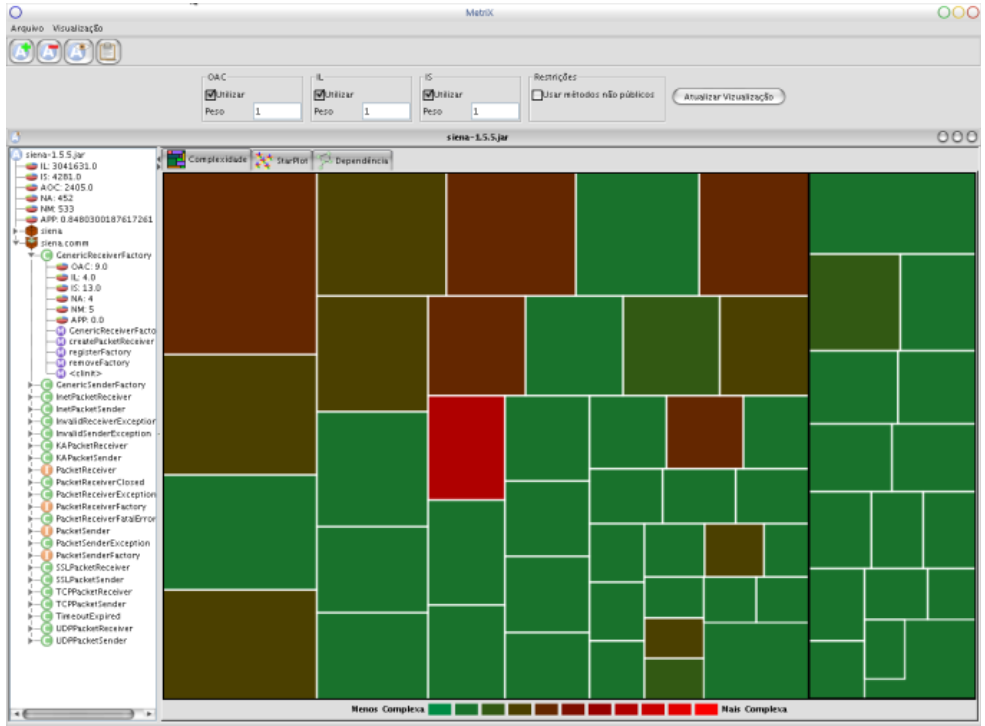
\includegraphics[width=0.8\textwidth]{Figures/tools/metrix.png}
  \caption[Visuelle Darstellung der Usability der Siena API]{Visuelle Darstellung der Usability der Siena API, \url{http://www.sienaproject.com/index.html} \citep{deSouza:ek}}
  \label{fig:metrix}
\end{figure}


\subsubsection{Concept Maps (Gerken u. a. 2011)}
\label{sec:concept-maps}
Die Verfahren wird von \cite{Tenny:2011jp} als longitudinaler Ansatz zur Bewertung von API Usability beschrieben. Der Terminologie von \cite{Sarodnick:2006vc} folgend, handelt es sich um eine empirisch-formativ-subjektive Evaluationsmethode.

Bei dieser Methode werden nicht nur einfache, sondern auch komplexe Problembewältigungen beobachtet, gemeinsam mit den Probanden besprochen und in Form einer auf einem Whiteboard festgehaltenen Concept Map dargestellt. Dazu treffen sich Experimentatoren und API-Anwender in regelmäßigen Abständen. Die API-Anwender werden aufgefordert, vorgegebene API-Konzepte und benutzerdefinierte Prototypkonzepte über benannte Kanten zu verbinden und existierende Verbindungen zu revisionieren. Problematische Bereiche können die API-Anwender rot umkreisen.
  
Über die Zeit entsteht nicht nur eine Abbildung der mentalen Modelle der API-Anwender, sondern auch eine Dokumentation, wie sich dieses Verständnis über die Zeit ändert. Nachteilig an diesem Verfahren ist, dass eine enge Zusammenarbeit zwischen API-Entwicklern und -Anwendern erforderlich ist. Dies setzt eine geographische Nähe wie auch eine hohe Bereitschaft und Offenheit auf beiden Seiten voraus.



\subsubsection{Guidelines / Best Practice}
Guidelines und Best-Practice-Zusammenstellung, wie die des Buches ``Effective C++: 50 Specific Ways to Improve Your Programs and Designs'' \citep{meyers1998effective}, stellen eine wertvolle Lektüre für API-Entwickler dar. Dennoch beschränken sich diese Ansätze eher auf das \textit{Wie}. Das \textit{Warum} wird allenfalls in Form von Usability-verschlechternden Gegenbeispielen dargestellt. Im Sinne einer API-Usability-Evaluation können derartige Aufzählungen als Checkliste verstanden werden, deren Verstoß vermutlich ein oder mehrere Usability-Probleme hervorrufen können. Für andere Sprachen wie Java \citep{bloch2008effective} gibt es ähnliche Werke.

\cite{Robillard:2010bh} stellt fest, dass die üblichen Guideline-Werke nicht viel mehr als Strukturierungstechniken gegen unbeabsichtigte Komplexität und Hinweise zur Namensgebung geben.
  
Aus meiner Sicht tragen Guidelines und Best-Practice am meisten dazu bei, einen Konsens zu etablieren und Konsistenz über viele APIs hinweg herzustellen, wodurch sich der Lernaufwand für API-Anwender mit jeder neuen API verringert.